% !arara: xelatex:  { action: nonstopmode, synctex: True }
% arara: biber
% !arara: makeglossaries
% arara: xelatex: {action: nonstopmode, synctex: True }
% arara: xelatex: {action: nonstopmode, synctex: True }

% A LANCER AVEC KNITR + xelatex

%NOTE POUR 2021 mettre à jour le fichier station pour inclure la Seiche
%%%%%%%%%%%%%%%%%%%%%%%%%%%%%%%%%%%%%%%%%%%%%%%%%%%%%%%%%%%%%%%%%%%%%%%%%%%%
%%%%%%%%%%%%%%%%%%%%%%%%%%%%%%%%%%%%%%%%%%%%%%%%%%%%%%%%%%%%%%%%%%%%%%%%%%%% 
%% 
%%  Scientific Report (Quick Draft) for LaTeX 
%%    By Andrej Korenic
%%    Tested in ScribTeX online and TeX Maker Version 3.1 (July 24th 2011)
%%    Created : November 2011
%%    Modified: 2023
%%
%%%%%%%%%%%%%%%%%%%%%%%%%%%%%%%%%%%%%%%%%%%%%%%%%%%%%%%%%%%%%%%%%%%%%%%%%%%%
%%%%%%%%%%%%%%%%%%%%%%%%%%%%%%%%%%%%%%%%%%%%%%%%%%%%%%%%%%%%%%%%%%%%%%%%%%%%
%%%%%%%%%%%%%%%%%%%%%%%%%%%%%%%%%%%%%%%%%%%%%%%%%%%%%%%%%%%%%%%%%%%%%%%%%%%%
%%
%%
%%
%% This file has content of the `elsarticle-template',
%% It is modified version by me, dedicated to scientists that want quick 
%% template for their scientific reports...
%%
%%
%% Copyright 2009 Elsevier Ltd (original copyright notes)
%%
%% This file is part of the 'Elsarticle Bundle'.
%% ---------------------------------------------
%%
%% It may be distributed under the conditions of the LaTeX Project Public
%% License, either version 1.2 of this license or (at your option) any
%% later version.  The latest version of this license is in
%%    http://www.latex-project.org/lppl.txt
%% and version 1.2 or later is part of all distributions of LaTeX
%% version 1999/12/01 or later.
%%
%%============================================================
%%============================================================
%% HOW TO USE IT
%%
%% All lines begining with %% are comments and they should stay
%% commented!!! Lines with only one % can be un-commented if you want
%% to use that function.
%%
%% Read instructions carefully!\documentclass[a4paper]{article}
%%============================================================
%%============================================================
%% DOCUMENT CLASS SETUP
%%
%% choose document class = type of the document...
%% Here you have Elsevier article, but you can override
%% page settings later!
\documentclass[10pt,twocolumn,titlepage,twoside]{article}\usepackage[]{graphicx}\usepackage[]{xcolor}
% maxwidth is the original width if it is less than linewidth
% otherwise use linewidth (to make sure the graphics do not exceed the margin)
\makeatletter
\def\maxwidth{ %
  \ifdim\Gin@nat@width>\linewidth
    \linewidth
  \else
    \Gin@nat@width
  \fi
}
\makeatother

\definecolor{fgcolor}{rgb}{0.345, 0.345, 0.345}
\newcommand{\hlnum}[1]{\textcolor[rgb]{0.686,0.059,0.569}{#1}}%
\newcommand{\hlsng}[1]{\textcolor[rgb]{0.192,0.494,0.8}{#1}}%
\newcommand{\hlcom}[1]{\textcolor[rgb]{0.678,0.584,0.686}{\textit{#1}}}%
\newcommand{\hlopt}[1]{\textcolor[rgb]{0,0,0}{#1}}%
\newcommand{\hldef}[1]{\textcolor[rgb]{0.345,0.345,0.345}{#1}}%
\newcommand{\hlkwa}[1]{\textcolor[rgb]{0.161,0.373,0.58}{\textbf{#1}}}%
\newcommand{\hlkwb}[1]{\textcolor[rgb]{0.69,0.353,0.396}{#1}}%
\newcommand{\hlkwc}[1]{\textcolor[rgb]{0.333,0.667,0.333}{#1}}%
\newcommand{\hlkwd}[1]{\textcolor[rgb]{0.737,0.353,0.396}{\textbf{#1}}}%
\let\hlipl\hlkwb

\usepackage{framed}
\makeatletter
\newenvironment{kframe}{%
 \def\at@end@of@kframe{}%
 \ifinner\ifhmode%
  \def\at@end@of@kframe{\end{minipage}}%
  \begin{minipage}{\columnwidth}%
 \fi\fi%
 \def\FrameCommand##1{\hskip\@totalleftmargin \hskip-\fboxsep
 \colorbox{shadecolor}{##1}\hskip-\fboxsep
     % There is no \\@totalrightmargin, so:
     \hskip-\linewidth \hskip-\@totalleftmargin \hskip\columnwidth}%
 \MakeFramed {\advance\hsize-\width
   \@totalleftmargin\z@ \linewidth\hsize
   \@setminipage}}%
 {\par\unskip\endMakeFramed%
 \at@end@of@kframe}
\makeatother

\definecolor{shadecolor}{rgb}{.97, .97, .97}
\definecolor{messagecolor}{rgb}{0, 0, 0}
\definecolor{warningcolor}{rgb}{1, 0, 1}
\definecolor{errorcolor}{rgb}{1, 0, 0}
\newenvironment{knitrout}{}{} % an empty environment to be redefined in TeX

\usepackage{alltt}
\usepackage{float}
\usepackage[section]{placeins}  %The placeins package provides the command \FloatBarrier
%%============================================================
%%============================================================
%% PACKAGE SETUP
\usepackage{fixltx2e} %textsubscript
%% Input and language packages.
\usepackage[T1]{fontenc}  %gestion des accents (pour les pdf) 
\usepackage{aeguill} % guillemets
%\usepackage[english]{babel}
\usepackage[french]{babel}
\addto\captionsfrench{\def\tablename{Tableau}}
\usepackage{amsmath} %equation
\usepackage{csquotes}
\usepackage{amsmath} %equation
\usepackage[math-style=ISO]{unicode-math}
\usepackage{microtype}
\setmainfont{Segoe UI}[
   Scale = 1.0,
   BoldFont = Segoe UI Semibold ,
   BoldItalicFont = Segoe UI Semibold Italic]
\setmathfont{Segoe UI}
\setmathfont{Asana-Math.otf}
\newfontfamily\titlefont{Georgia} 
%% Parskip is the extra vertical space inserted before a paragraph. It has a natural length of zero but should be a rubber length so that it may be stretched in a flushbottom environment. To increase \parskip to skip a line between paragraphs one could use \addtolength{\parskip} {\baselineskip}.
\usepackage{parskip}
\usepackage{latexsym} % pour les carrés
%% Sets space between lines.
\usepackage{setspace} 
%\usepackage{supertabular}
\usepackage{siunitx,booktabs}
\usepackage{caption} % pour éviter les problème de place entre le header et le tableau
\captionsetup[table]{skip=5pt}

%% If you use PostScript figures in your article
%% use the graphics package for simple commands
%\usepackage{graphics}
%% or use the graphicx package for more complicated commands (places the float at precisely the location in the LaTeX code [H]).
\usepackage{graphicx} \usepackage{float}
%% or use the epsfig package if you prefer to use the old commands.
%\usepackage{epsfig}

%% Using captions in floating environment. Note: might not work with other packages.
%\usepackage{caption}

%% Making numbered and bulleted lists.
\usepackage{enumerate}

\usepackage{xcolor} % Required for specifying colors by name
\definecolor{bleu_EV}{RGB}{0,33,143}
\definecolor{turquoise_EV}{RGB}{0,201,196}
\definecolor{orange_EV}{RGB}{255,117,87}
\definecolor{jaune_EV}{RGB}{255,180,40}
\definecolor{bleuazur}{RGB}{48,113,162}
\definecolor{marron}{RGB}{70,40,0}
\definecolor{bleu_EVf}{RGB}{0,19,80}
\definecolor{jaune_EVf}{RGB}{173,112,0}
\definecolor{turquoise_EVf}{RGB}{0,120,115}
\definecolor{orange_EVf}{RGB}{178,81,60}
\definecolor{bleu_clair_EV}{RGB}{51,181,255}

%% Math packages
%\usepackage{amsmath, amssymb}

%% The amsthm package provides extended theorem environments.
%\usepackage{amsthm}

%% The verbatim environment, \begin{verbatim} ... \end{verbatim}, permits us to insert large sections of reformatted text in a LaTeX file (including block of comments). It is very handy for inserting large chunks of code in a document, for example, literal TeX code or the Maple code you sweated over and now want to comment on.
%\usepackage{verbatim}

%% Add hyperlinks, so that you can click on references, theorem numbers etc. to jump to the place where they are in the paper (at least for the DVI and PDF versions), it seems that \documentclass{article} does not work with hyperref; use instead \documentclass{amsart}. Note: first test it with Elsevier template!
\usepackage{hyperref} 
\hypersetup{pdftex, 
colorlinks=true, 
linkcolor=orange_EVf, 
citecolor=orange_EV, 
filecolor=bleu_EV, 
urlcolor=bleu_EV, 
pdftitle= {Suivi de l'anguille jaune (\textit{Anguilla anguilla}, L.) en pêche
électrique sur le bassin de la Vilaine de 1998 à 2024.},
pdfauthor={Cédric Briand}, pdfsubject={anguille},
pdfkeywords={anguille} {pêche électrique} {marquage} }



%% The numcompress package shorten the last page in references.
%% `nodots' option removes dots from firstnames in references.
%\usepackage[nodots]{numcompress}

%% The lineno packages adds line numbers. Start line numbering with
%% \begin{linenumbers}, end it with \end{linenumbers}. Or switch it on
%% for the whole article with \linenumbers after \end{frontmatter}.
%% \usepackage{lineno}

%% If you are printing how many pages you submitted...
\usepackage{lastpage}

%% The \url{...} command does all the work: It sets the enclosed expression in the appropriate typewriter style font, it takes care of any necessary linebreaking, and it chooses break points intelligently (e.g., between components of an address), and it ensures that special symbols such as the tilde symbol or the "at" symbol get typeset correctly.
\usepackage{url}

%% A new implementation of LATEX's tabular and array environment.
 \usepackage{array}
 
\usepackage{longtable}



%%============================================================
%% BIBLIOGRAPHY SETUP
%%============================================================
\usepackage[style=authoryear, %numeric
            natbib=true, % citep and citet
            backend=biber, % default for biblatex
            bibencoding=utf8,
            url=false, 
            doi=false,
            firstinits=true, % pas de prenoms
            %sorting=nyt, % name, year, title
            eprint=false]{biblatex} % option natbib to use cite and citep
\addbibresource{pechelec.bib}



%%============================================================
%%============================================================
%% PAGE SETUP

	%% Easier way...
	\usepackage[a4paper, inner=1.5cm, outer=1.5cm, top=2cm, bottom=3cm]{geometry}
	%% The hard way involves setting all the desired values manually. Here are some values that can be set: 
	%% Dimensions of the PDF file.
	%\pdfpageheight \pdfpagewidth
	%% Length of margin at top of page above all printing. 1 inch is added to this value.
	%\topmargin   
	%% Left margin on even numbered pages. 1 inch is added to this value.
	%\evensidemargin  
	%% Left margin on odd numbered pages. 1 inch is added to this value.
	%\oddsidemargin
	%% Height of the page header.
	%\headheight
	%% Distance from bottom of header to the body of text on a page.
	%\headsep
	%% Distance from top of main text box to the baseline of the first line of text in the Fetmain text box.
	%\topskip 
	%% Height and width of main text box.
	%\textheight \textwidth
	%% Distance from bottom of body to the bottom of the footer.
	%\footskip
	%% Distance between paragraphs.
	%\parskip
	%% Amount of indentation at the first line of a paragraph.
	%\parindent
	%% Uncomment if don't want page numbers.

%----------------------------------------------------------------------------------------
%	PAGE HEADERS (this must come after loading and setting geometry)
%----------------------------------------------------------------------------------------

\usepackage{fancyhdr} % Required for header and footer configuration

\pagestyle{fancy}

% Chapter text font settings
\renewcommand{\sectionmark}[1]{\markright{\sffamily\normalsize\thesection\hspace{5pt}#1}{}}
%\renewcommand{\subsectionmark}[1]{\markboth{}{\sffamily\normalsize\thesubsection\hspace{7pt}#1}}
% Section text font settings
\fancyhf{} \fancyfoot[C]{\sffamily\normalsize\thepage} % Font setting for
% the page number in the header
\fancyhead[LE,RO]{\sffamily \rightmark}
\fancyhead[LO,RE]{\slshape \normalsize Rapport pêche électriques 2024}






%%============================================================
%%============================================================
%% DEFINING NEW COMMANDS AND ABBREVIATIONS
%% Use this section to define new commands that you will use in
%% your report.

%% Makes a path to your graphics' folder.
\graphicspath{{C:/workspace/pechelec/image/2024/}}

\usepackage[most]{tcolorbox} % summary at the end


%% Add extra space to multi-line equation environments
%\setlength{\jot}{9pt}

% use \mbox{...} for no separation of the defined word
\usepackage[explicit]{titlesec} % explicit says you must use #1 below
% \titleformat{hcommandi}[hshapei]{hformati}{hlabeli}{hsepi}{hbefore-codei}[hafter-codei]
\newlength\secnumb
\setlength\secnumb{2cm}
%https://borntocode.fr/latex-personnaliser-les-titres-chapter/
\titleformat{\section}[block]  %display et frame. La première est celle
% utilisée par défaut par les titres de latex, elle sépare le titre du prochain paragraphe. La seconde permet d’ajouter un cadre autour du titre
    {\LARGE\textcolor{bleu_EV}\titlefont}
    {}
    %hformati is the format to be applied to the whole title—label and text.
    % This part can contain vertical material (and horizontal with some shapes) which is typeset just after
    %the space above the title.
    {0pt} %hsepi is the horizontal separation between label and title body and
    %must be a length (it must not be empty). This space is vertical in display
    % shape; in frame it is the distance from text to frame. Both hlabeli and hsepi are ignored in starred versions of sectioning
    %commands. If you are using picture and the like, set this parameter to 0
   % pt.
    { 
     \parbox[b]{\secnumb}{
      \fontsize{50}{60}\selectfont\titlefont\textcolor{bleu_EV}{\thesection}}
      % {1} must be 1.2 {2}
      \parbox[b]{\dimexpr\columnwidth-\secnumb-2em\relax}{
        \raggedleft
        \hfill{\LARGE\titlefont\textcolor{bleu_EV}{#1}}\\
        \textcolor{bleu_EV}{\rule{\dimexpr\columnwidth-\secnumb-2em\relax}{0.4pt}}
        }}
    
 % pour les chapitres sans numéro
 %Both hlabeli and hsepi are ignored in starred versions of sectioning
%  commands. 
\titleformat{name=\section,numberless}[block]  
    {\LARGE\textcolor{bleu_EV}\titlefont}
    {}
    {0pt} 
    {\parbox[b]{\chapnumb}{%
   \mbox{}}%
    \parbox[b]{\dimexpr\columnwidth-\secnumb-2em\relax}{
        \raggedleft
        \hfill{\LARGE\titlefont\textcolor{bleu_EV}{#1}}\\
        \textcolor{bleu_EV}{\rule{\dimexpr\columnwidth-2em\relax}{0.4pt}}
        }%
     }
\titleformat{\subsection}[display]    % hand is the default for sections but use display to avoid par extending over the margin
        {\Large\titlefont}
        {\textcolor{bleu_EV}
        {\subsectiontitlename \thesubsection \quad #1}}
        {0pt}
        {}
\titleformat{\subsubsection}[display]    % hand is the default for sections
        {\titlefont}
        {\textcolor{bleu_EV}
        {\subsubsectiontitlename \thesubsubsection \quad #1}}
        {0pt}
        {}
        
%\titlespacing*{<command>}{<left>}{<before-sep>}{<after-sep>}
\titlespacing*{\section}{0}{4.5ex plus 1ex minus .2ex}{3.3ex plus .2ex}
\titlespacing*{\subsection}{0}{3.5ex plus 1ex minus 1ex}{1ex plus .2ex}
\titlespacing*{\subsubsection}{0}{2.5ex plus 1ex minus 1ex}{0.5ex plus .1ex}
%%===============================================%%
%%==========    END OF THE PREAMBLE    ==========%%
%%===============================================%%



%%============================================================
%%============================================================
%%============================================================
% BEGINNING OF THE TEXT BODY

%% You can write here small footer that will go on the first page, together with
%% the date stamp; comment the line if you don't want that!
%\footme{Submitted to Someone Somewhere\hspace{2mm}(\pageref{LastPage} pages)} \datestamp{Andrej Korenic, 27$^{th}$ October, 2011}
\IfFileExists{upquote.sty}{\usepackage{upquote}}{}
\begin{document}


\newpage
\newgeometry{right=1.5cm, left=1.2cm, top=0.2cm, bottom=2cm}
\thispagestyle{empty}
\pagecolor{bleu_EV}
\newgeometry{margin=0cm}
\begin{minipage}{\textwidth}
\vspace{30pt}
\hspace{30pt}
\includegraphics[width=6cm,keepaspectratio=true]{/logo_EV1}
\end{minipage}

%\vspace*{0cm}
\begin{minipage}{0.1\textwidth}
\phantom{This text will be invisible}
\end{minipage}
\begin{minipage}{0.8\textwidth}
\begin{center}
\noindent
{\color{turquoise_EV}\rule{\textwidth}{2.5pt}}\\
\vspace{8mm}
\color{white}
\color{white}
{ \titlefont \huge  \bfseries{Suivi de l'anguille jaune (\textit{Anguilla anguilla}, L.) en pêche
électrique sur le bassin de la Vilaine de 1998 à 2024\\
    }}
\bigskip
{\titlefont  \LARGE rapport 2022-2024\par }
\vspace{4mm}\noindent
{\color{turquoise_EV}\rule{0.9\textwidth}{1.8pt}}\par
\vspace{5mm}
{\color{jaune_EV}{\Large \itshape{Léa Patau, Cédric Briand,
      Brice Sauvaget,
      Gérard Eriau\par   }}}
\end{center}
\end{minipage}



\vspace{2cm}%

\begin{minipage}{\textwidth}
\begin{center}
 \rotatebox{270}{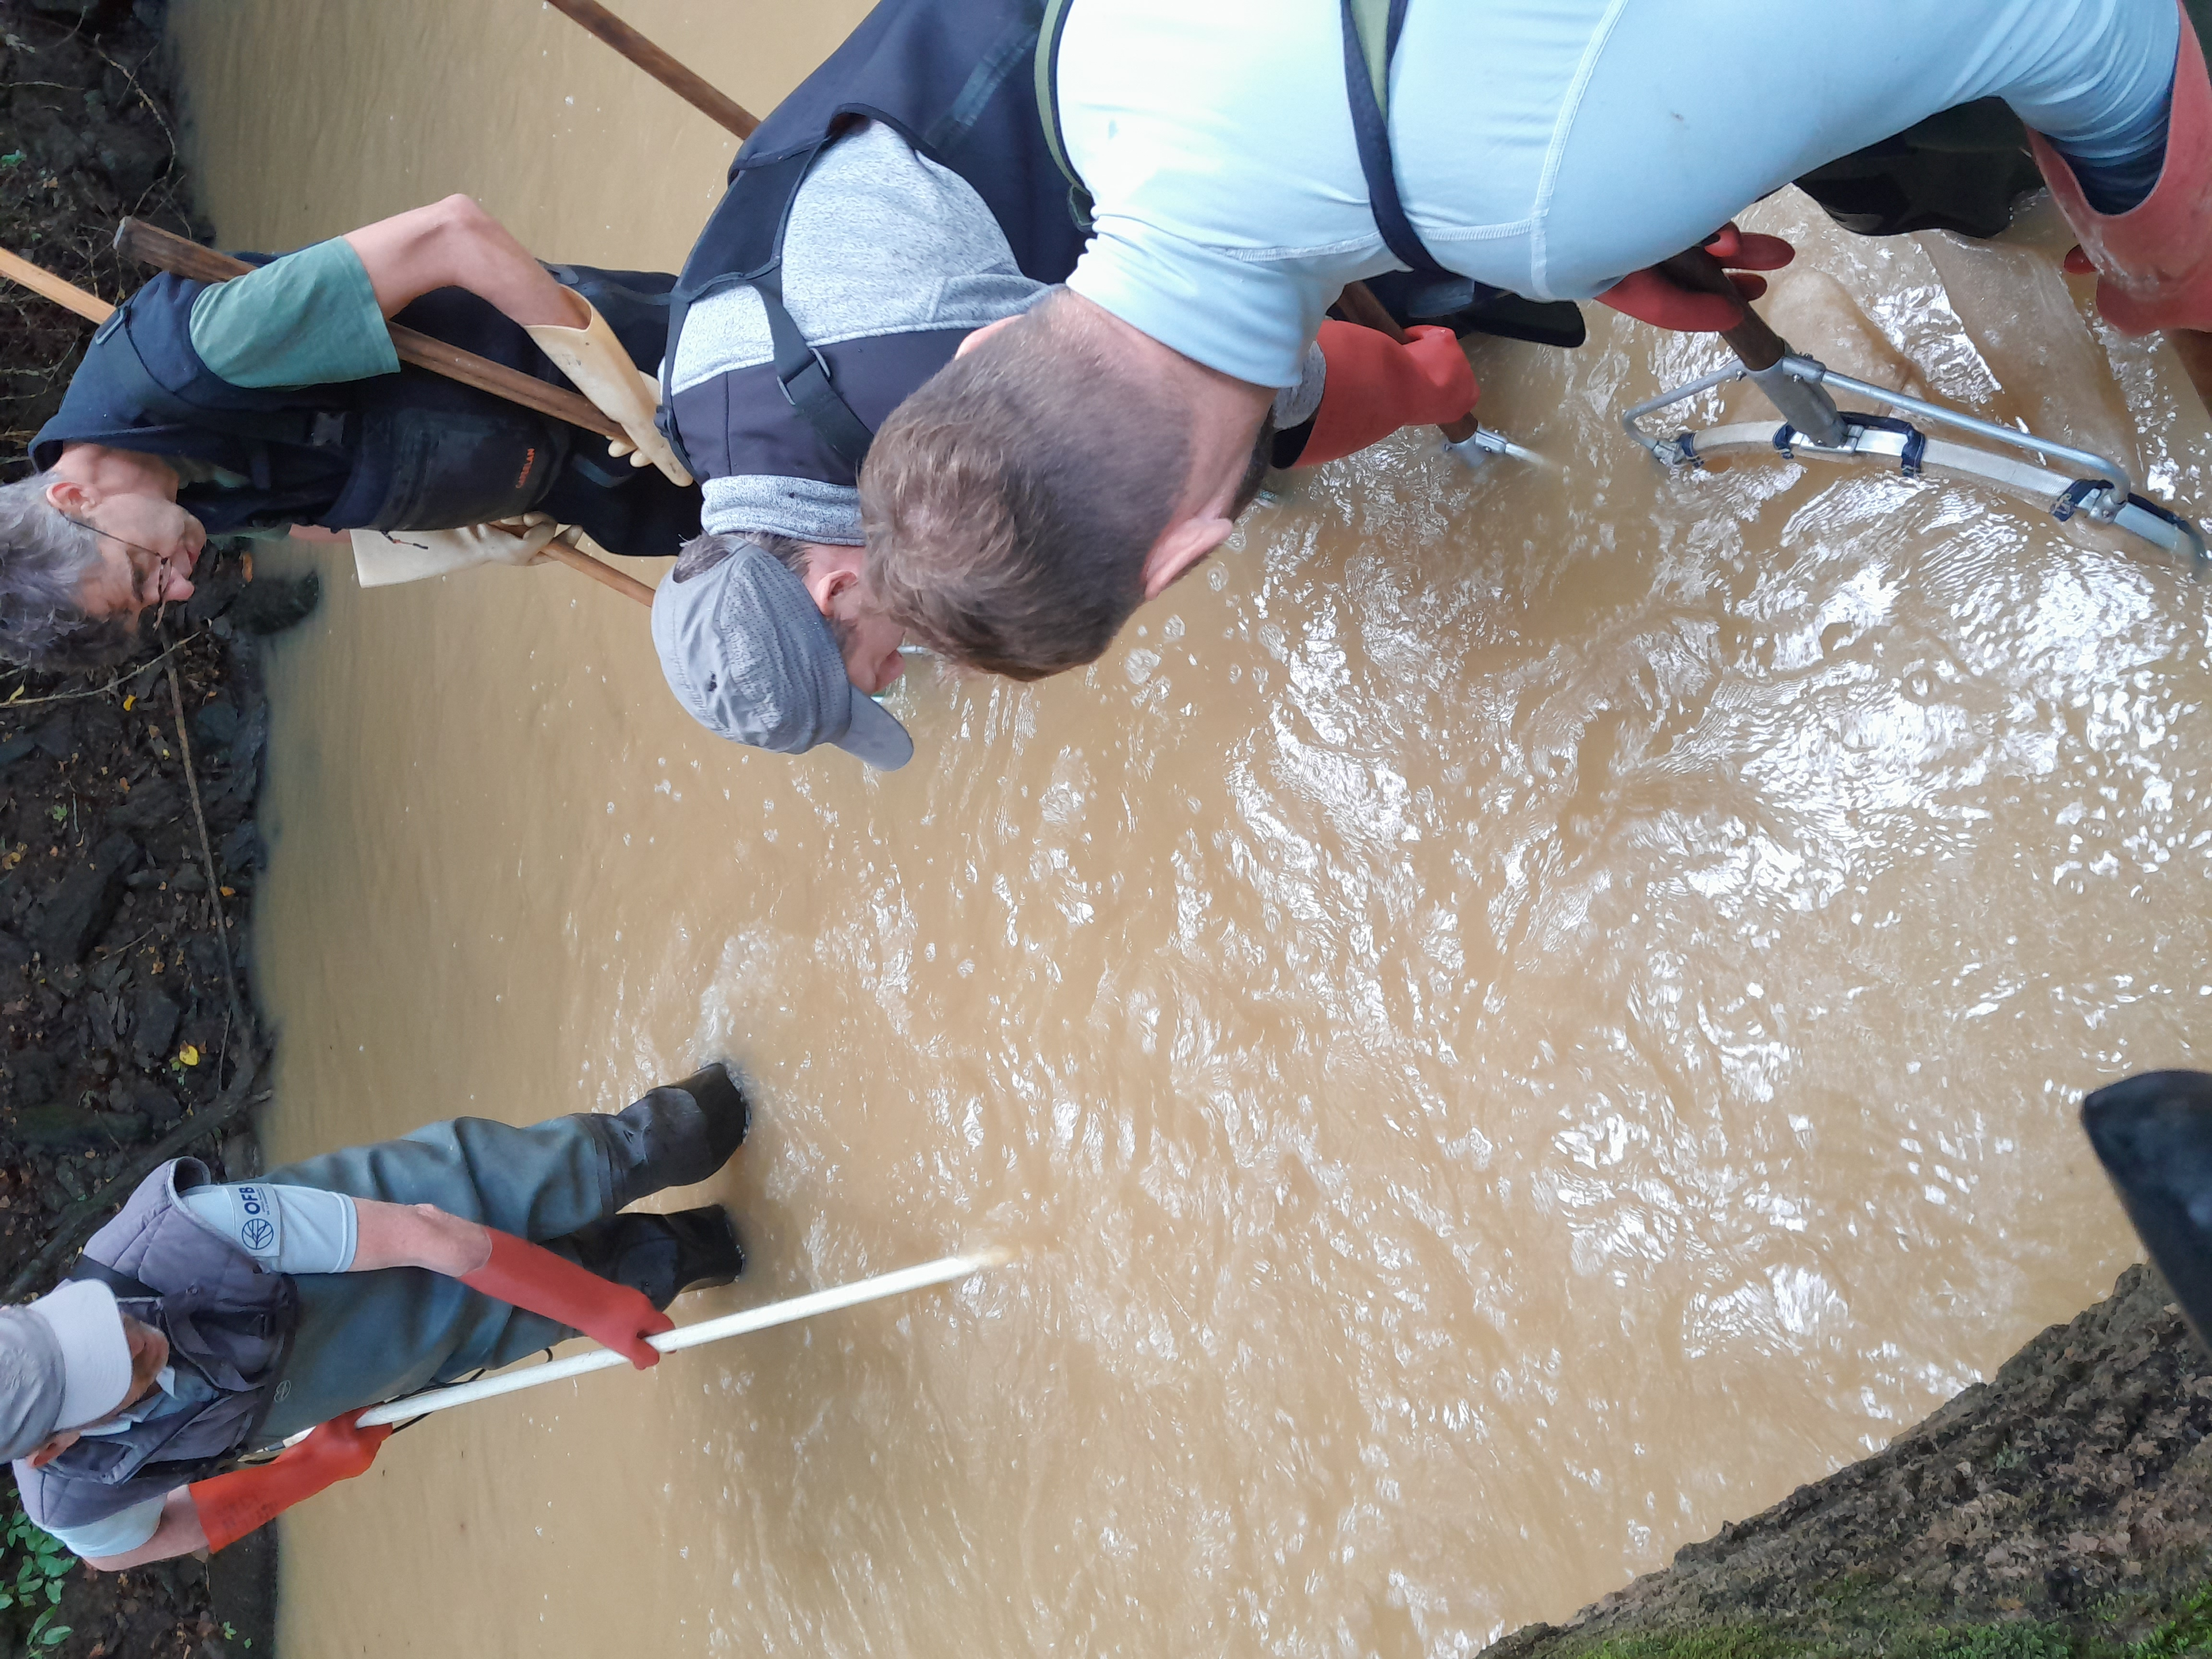
\includegraphics[width=0.5\paperwidth]{../peche.jpg}}
\end{center}
\end{minipage}

\vspace{2cm}%

\begin{minipage}{0.8\textwidth}
\begin{center}
\hspace{3cm}{\color{white}{\huge \itshape{Mars 2024}}}
\end{center}
\end{minipage}
\restoregeometry
\clearpage
\normalsize
\pagecolor{white}



%---------------------------------------------------------------------

%% Switch on the line numbers for the whole article at this place.
%\linenumbers

%% Here you can put your table of contents and also give it a new name.		
\newpage
\renewcommand{\contentsname}{Sommaire:}
\tableofcontents

%% Switch on the line numbers for the whole article at this place.
%\linenumbers

%% Main text is going here.

\bigskip


\section{Matériel et méthodes}



%
%
Pour cette étude, le bassin versant a été séparé en trois
classes de distance (rkm = kilomètres de rivière) :
\begin{description}
\item [la zone aval] située
à moins de 50 kilomètres de rivière du barrage
d'Arzal (50 rkm) est formée principalement
par des affluents connectés au bief aval de la Vilaine sous influence
directe du barrage d'Arzal. Le cours principal de la
Vilaine forme un bief de 30-150 m de large, en connexion avec les
marais de Redon.
\item [la zone intermédiaire] est composée de secteurs
situés entre 50 et 100 kilomètres de rivière du barrage
d'Arzal (50-100 rkm). Les affluents échantillonnés
comportent le Canut Sud, séparé de la Vilaine aval par un barrage,
et le ruisseau de l'Aron accessible après deux
barrages. Le troisième, le ruisseau des Arches, est plus difficile
d'accès pour les anguilles. Il est localisé sur
l'Oust et est séparé par 6 barrages de navigation
de la Vilaine aval. Cet axe a été entièrement équipé de
passes à anguilles en 2003.
\item [la zone amont] (100 rkm) comprend des affluents connectés à
l'axe de la Vilaine. Les points
d'échantillonnage sont localisés entre 110 et 165
kilomètres du barrage d'Arzal. En 1999 et 2000, 13
passes à anguilles ont été construites sur les barrages de
navigation de la Vilaine, facilitant l'accès aux
affluents du Canut Nord et de la Chèze. Elles ont aussi facilité
l'accès au Chevré situé en amont de Rennes, bien
que trois barrages soient restés non équipés pour
l'accès à cette rivière. Une passe à anguilles
située sur le troisième barrage de la Vilaine (la Molière) a
été arrachée durant la crue de l'hiver 2000 et
reconstruite en 2006.
\end{description}
\begin{figure}[htbp]
\centering
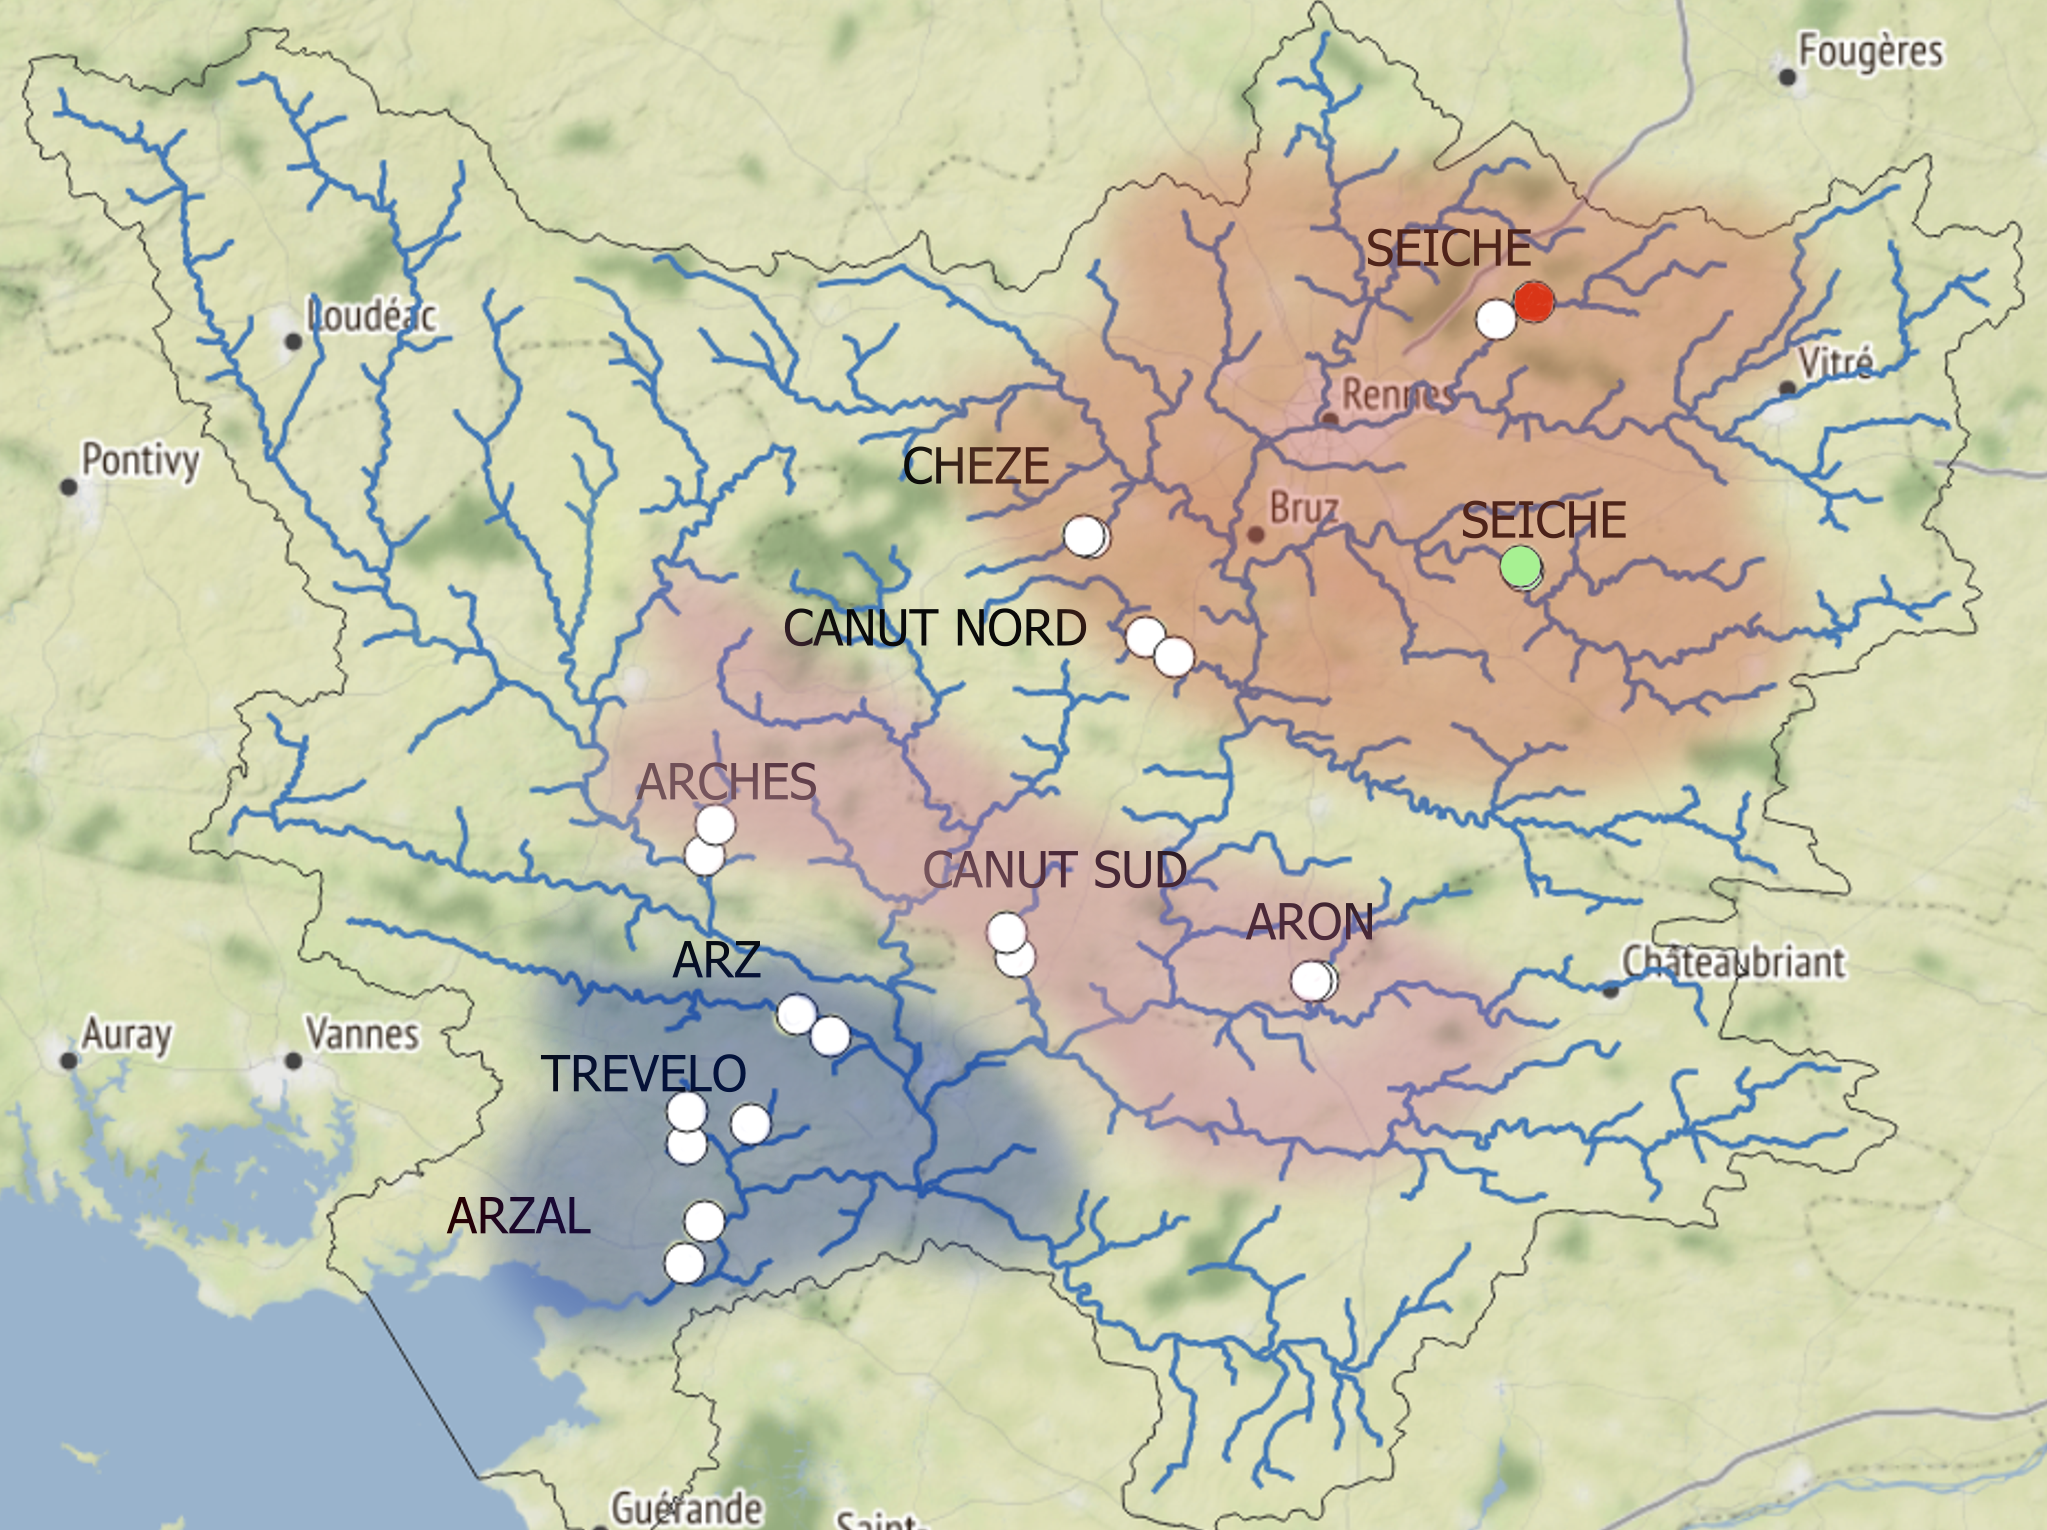
\includegraphics[width=0.5\textwidth]{../carte2021_1.png}
\caption[Vue schématique du bassin de la Vilaine]{Vue schématique du bassin de
la Vilaine, les trois zones colorées correspondent aux trois classes de
distance de l'estuaire, <50 rkm, 50-100, >100 rkm. La station du Chevré
abandonnée en 2020 est en rouge, les 2 nouvelles stations de la Seiche sont en
vert. }
\label{fig_carte}
\end{figure}
%
\subsection{Méthode de pêche}
%
Sur 46 stations de pêche électrique
prospectées sur le bassin versant de la Vilaine chaque année entre
fin août et novembre de 1998 à 2005
(BRIAND \textit{ et
al.}, 2006), une sélection de 19 stations
situées sur 10 affluents a été conservée à partir de 2007
(Figure \ref{fig_carte}). La
méthode de pêche est standardisée. Les pêches électriques
sont effectuées à l'aide d'un
matériel de type Héron. Le courant utilisé est continu. Les secteurs de pêche
couvrent approximativement une surface de pêche de 100 m$^2$.
Ils sont délimités et marqués de manière à prospecter le
même secteur d'une campagne de pêche sur
l'autre. Une attention particulière a été portée à la continuité des
équipes de pêche depuis le début des opérations et que le protocole de pêche
soit équivalent d'une année sur l'autre.
L'anode est placée à intervalles réguliers de
manière à prospecter l'ensemble de la surface du
secteur de pêche. Une fois le courant appliqué,
l'électrode est maintenue en place pendant au minimum
30 secondes, plus si une anguille détectée n'est
pas encore capturée. La capture des anguilles est effectuée par
deux pêcheurs, équipés d'une épuisette large
à cadre métallique avec le bord inférieur droit de 60 cm de large
avec des mailles de 2 mm ; et d'une petite épuisette
à main ronde ou carrée avec des mailles de 2 mm. Cet équipement
peut varier en fonction des circonstances. Les grandes épuisettes
sont surtout efficaces dans les secteurs où le débit est important
et la visibilité réduite. Lorsque le débit est faible ou nul, les
grandes épuisettes ne sont pas utilisées. Les épuisettes
secondaires peuvent être remplacées par des petites épuisettes
rectangulaires utilisées dans la biométrie lorsque le cours
d'eau pêché est en étiage sévère, et
qu'il est nécessaire de
 \og chasser \fg les anguillettes dans les
interstices des pierres sur les radiers. Les stations pêchées font
l'objet d'un inventaire complet de la
faune piscicole présente. Le nombre d'anguilles
collectées par point est noté par un opérateur en rive, qui est
également chargé de contrôler le temps de pêche.
%
\subsection{Traitement des données}
Les migrations vers le fleuve sont analysées en faisant la somme :
\begin{itemize}
\item des montées de civelles aux passes,
\item des migrations d'anguilles jaunes,
\item des opérations de transport qu'elles soient effectuées par l'IAV ou par le
CRPMEM. Dans tous les cas, les mortalités lors des transports ne sont pas
inclues,
\item des migrations dans l'écluse.
\end{itemize}

Les densités sont évaluées comme suit :
\begin{equation*}
D=\frac{N_{CS}}{surface}
\end{equation*}
où $N_{CS}$ correspond aux nombres évalués par la
méthode des enlèvements successifs de Carle \& Strubb
\citep{ogle_fsa_2013,carle_new_1978} à partir des effectifs pêchés sur chaque 
station $N$ et la surface correspond à la surface mouillée de la
station de pêche.\\

L'efficacité de pêche $\Phi$ est calculée à partir de l'effectif
Carle\&Strubb $N_{CS}$ et de l'effectif au premier passage
$N_{p1}$ :
\begin{equation*}
\Phi=\frac{N_{p1}}{N_{CS}}
\end{equation*}
Les biomasses d'anguilles estimées
$B_e$
par station sont calculées à partir des biomasses :
\begin{equation*}
B_e=B\times \frac{D}{N}
\end{equation*}

Les densités de chaque classe de taille $\tau$ sont calculées comme
suit :

\begin{equation*}
 D_{\tau}=N_{\tau} \times \frac{N_{CS}}{N \times surface}= N_{\tau} \times \frac{D}{N}
\end{equation*}


Les densités par classe d'âge sont calculées grâce à la clé
taille-âge élaborée par Mounaix \citep{mounaix_intercalibration_1992} complétée par
des anguilles prélevées en 1998 et 1999 dans les cours
d'eaux \citep{briand_effect_2006}.
%
\subsection{Analyses statistiques}
%
Les densités d'anguilles sont log transformées pour
normaliser la distribution (Shapiro-Wilks p{\textgreater}0.1). Une
analyse est appliquée en utilisant la formule :
\begin{equation*}
\log (D){\approx}a+s+m+\epsilon_s
\end{equation*}
pour laquelle la station $s$ correspond à la station de pêche, le mois $m$
correspond au mois divisé en deux catégories avant septembre et après octobre,
et l'année $a$ correspond à l'année de pêche. Un modèle linéaire simple montre
que les variances des résidus sont différentes entre les stations. Les
 données sont donc analysées par un modèle linéaire mixte
 \citep{pinheiro_nlme_2013} avec un lien identité et une distribution normale, 
 pour lequel une variation de la variance en fonction de la station est appliquée $\epsilon_s=N(0,{\sigma_{s}}^2)
~s=1,\dots,19$ \citep{zuur_mixed_2009}. La significativité des différentes
variables -classe de distance à la mer, affluent, station ou mois- est évaluée à
l'aide du critère d'Akaike (AIC) ou du ratio des log-vraissemblance lorsque les modèles sont structurellement emboîtés. Un test
post hoc de Tukey est appliqué aux densités pour grouper les années semblables.
L'évolution de la densité en anguilles et des biomasses est analysée par zone (classe de
distance du barrage) et par âge. Les tendances de densité sont analysées ainsi
que la moyenne par secteur de distance. Cette moyenne est comparée à la valeur de référence de 0.3
anguille.m$^{-2}$ indiquée par le PLAGEPOMI pour les parties aval des cours
d'eaux.
%
\subsection{Marquage recapture des anguilles}
%
A partir de 2009, le marquage des anguilles a été effectué par pit tag à l'aide
d'un injecteur manuel sur toutes les anguilles de plus 30 cm capturées sur les stations. Les
pits tags ont été placés dans la cavité abdominale.
Ils sont passés dans une solution de chlorhexidine diluée à 0.5 \% dans l'eau 
avant d'être
implantés.
Les anguilles de taille susceptible d'être recapturées après avoir été marquées > 30 cm ont été testées pour le marquage. 
Sur certaines stations, une prospection est effectuée en dehors de la station
pour rechercher les anguilles de plus de 30 cm et vérifier si elles ont déjà
été marquées.
Ces anguilles sont alors traitées à part dans les données de pêche mais sont intégrées aux stations de pêche.


\section{Résultats}


\subsection{ Recrutement estuarien}


Les captures totales de la pêcherie sont passées de 57 tonnes en
1981 à  2.6 tonnes en 2009 et sont remontées autour de 4 à 6 tonnes
après 2015 (Tableau \ref{tableau_captures}).
Avant l'adoption du plan de gestion, les captures étaient essentiellement contraintes par la durée de la saison de pêche
\citep{briand_dynamique_2009}. Après cette date, elles sont plus le reflet des
contraintes du quota et du marché pour la civelle, avec la fermeture à l'export
par la CITES à partir de 2010. La fermeture de la pêche est intervenue plus tôt
dans la saison après 2018.
\small
\begin{table}[htpb]
\centering
\caption{Captures de la pêcherie de civelles d'Arzal de 1995 à 2024, sources : 
1= Affaires Maritimes (données mareyeurs), 
2= De Casamajor \& Briand 2009 (OFIMER),
3= Comité des pêches maritimes Auray-Vannes,
4=télécapêche Vilaine (Comité des pêches maritimes Auray-Vannes). 
La date d'arrêt correspond à la date de fermeture de la pêche en fin de saison.}
\label{tableau_captures}
\begin{tabular}{llll}
\toprule
Année & Capture (t) & Source & Arrêt \\ 
\midrule
1995  & 29.50  &  1 & 30-avr \\
1996  & 22.40  &  1 & 15-avr \\
1997  & 22.60  &  1 & 30-avr \\
1998  & 17.50  &  1 & 06-avr \\
1999  & 14.93  &  1 & 05-avr \\
2000  & 13.94  &  1 & 15-avr \\
2001  & 7.93   &  1 & 30-mars \\
2002  & 14.51  &  1 & 23-mars \\
2003  & 9.14 &  1   & 23-mars \\
2004  & 7.26 &  1  & 27-mars \\
2005  & 6.72 &  1  & 20-mars \\
2006  & 6.99 &  1  & 23-mars \\
2007  & 6.78 &  1  & 11-mars \\
2008  & 4.57 (4.2) & 3 (2) & 11-mars\\
2009  & 2.61 & 3  & 31-mars \\
2010  & 3.03 & 3 & 30-avril \\
2011  & 3.92 & 3  & 30-avril \\
2012  & 2.99 & 3  & 30-avril \\
2013  & 2.10 & 4  & 30 avril \\
2014  & 2.68 & 4  & 30 avril \\
2015  & 4.86 & 4  & 30 avril \\
2016  & 4.62 & 4 &  30 avril\\  % j'ai mis la valeur par défaut, mais je n'ai pas la valeur dans le tableau
2017  & 5.87 & 4  & 30 avril \\ 
2018 & 6.53 &  4  & 30 avril \\ 
2019 & 5.13 &  4  &  14 mars\\ 
2020 & 3.45 &  4  &  22 mars \\ 
2021 & 4.53 &  4  &  17 mars \\
2022  & 5.40 & 4 & 19 mars \\ 
2023  & 4.68 & 4 & 17 mars \\
2024  &      &   &  TODO  \\
\bottomrule
\end{tabular}
\end{table}
\normalsize
\subsection{Recrutement fluvial}




Le recrutement fluvial vers le bassin versant
est composé majoritairement du stade civelle, variant annuellement de
$0.026$ en 2010 à
$7.044$ millions de civelle par an en 
2013. 
Le nombre d'anguilles jaunes comptées sur les passes a varié de
$878$ à  $144~992$
entre la plus mauvaise année 2005 et la meilleure
2013. Les données reportées pour le recrutement
d'anguilles jaunes sur le bassin sont présentées différemment avec un calcul par
cohorte, qui prend en compte l'âge des anguilles lors de leur passage. Les
effectifs d'anguilles jaunes varient alors entre
$6~350$ et $160~669$ 
(Figure \ref{figure2recrutement}) \citep{briand_gestion_2017}.
Entre 2000 et 2005, les captures lors des pêches expérimentales pour
transfert en amont du barrage ont lissé la chute du recrutement fluvial sans la
compenser pleinement (Figure \ref{figure2recrutement}). L'augmentation de la
migration des anguilles jaunes après 2005 est concomitante avec
l'arrêt des pêches scientifiques de civelles
après la saison de pêche professionnelle (en bleu sur la Figure
\ref{figure2recrutement}). Les variations des migrations de civelles sur la
passe (Figure \ref{figure2recrutement}) sont essentiellement la conséquence du taux
d'exploitation des civelles en estuaire.
Après 2012, les variations du recrutement fluvial reflètent les tendances du
recrutement (Figure \ref{figure_recrutement}), les transports, les variations
du taux d'exploitation de la pêcherie, et les manoeuvres d'écluse au barrage
d'Arzal. En pratique, le recrutement fluvial est aujourd'hui proche des
niveaux faibles observés entre 2000 et 2005. La même figure est reportée en kg
pour les civelles (Figure \ref{figure2recrutement_kg}).
Entre 1996 et 2005, \citet{briand_dynamique_2009} a estimé l'efficacité de la
passe entre 3 et 16\% à l'aide d'opérations de marquage-recapture. En faisant
l'hypothèse d'une efficacité de la passe de 10 \% après 2005, le taux
d'exploitation annuel de la pêcherie varie entre 22.7\% (2012--2013) et 98.1\%
(2009-2010). Les deux dernières années le taux d'exploitation serait remonté autour de 79\%
(2019--2020) et 83 \%. En moyenne, il est de 67\% et ce taux est donc supérieur
à la cible de gestion fixée par le règlement européen (40 \% d'échappement soit
60\% de taux d'exploitation). Une telle cible de gestion ne serait appliquable
que si on avait restauré le stock et qu'aucune autre mortalité anthropique
(turbines, pêche amateur au stade jaune) n'était appliquée à l'anguille au
cours de son cycle de vie.
Il faut noter que pour le rapportage, le taux d'exploitation n'est évalué qu'à l'échelle 
de l'unité de gestion (Bretagne), et que même pour la phase civelle, il est
beaucoup plus faible car les pêcheries de civelles sont par ailleurs beaucoup
plus limitées en Bretagne.



\begin{figure}[htbp]
\centering
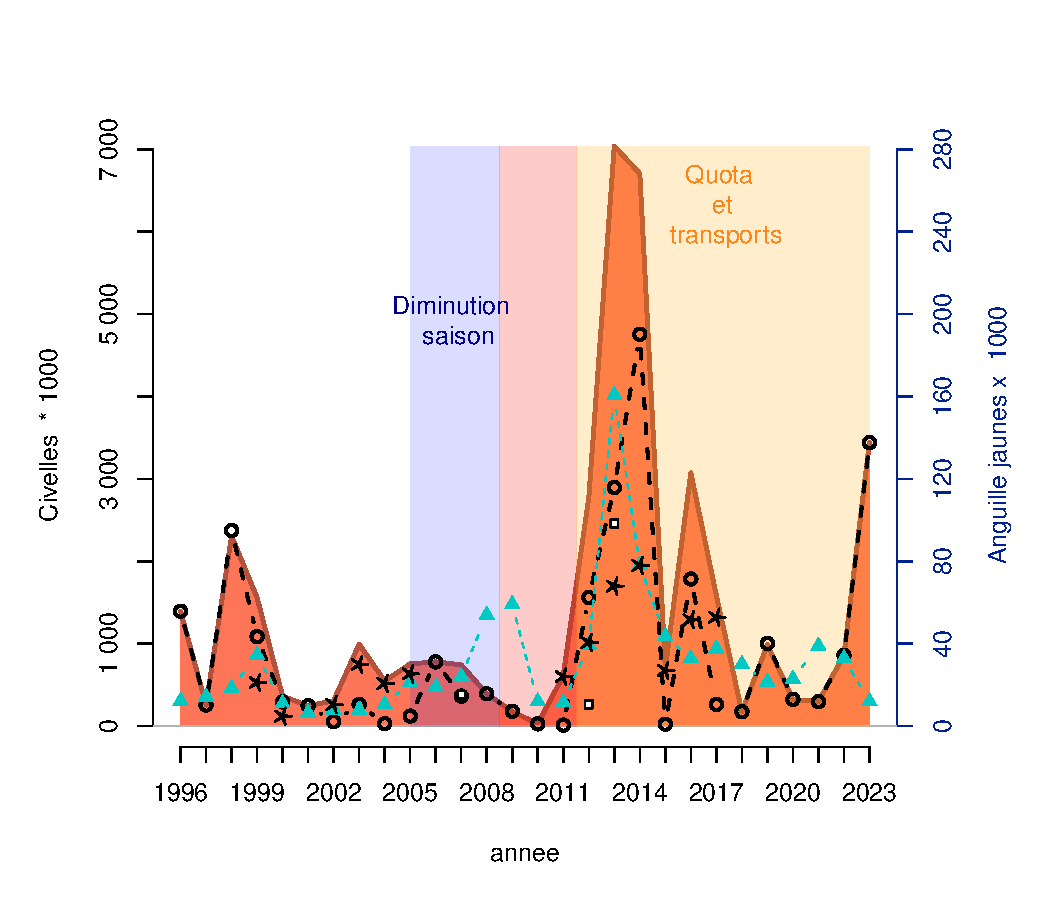
\includegraphics[width=0.5\textwidth]{figure2recrutement.pdf}
\caption[Tendance des densités modèle]{Migrations d'anguilles
jaunes (ramenées à leur cohorte d'arrivée) (\textmd{{}-{}-${\Delta}$-{}-}) et de civelles
(\textmd{{}-}o\textmd{{}-}) en effectif sur la passe au barrage d'Arzal,
civelles pêchées et transportées ($\star$) et estimation de la migration de civelles
lors des man{\oe}uvres d'écluse entre 1996 et 2011 ($\Box$). En orange, somme du
recrutement fluvial de civelles.}
\label{figure2recrutement}
\end{figure}

\begin{figure}[htbp]
\centering
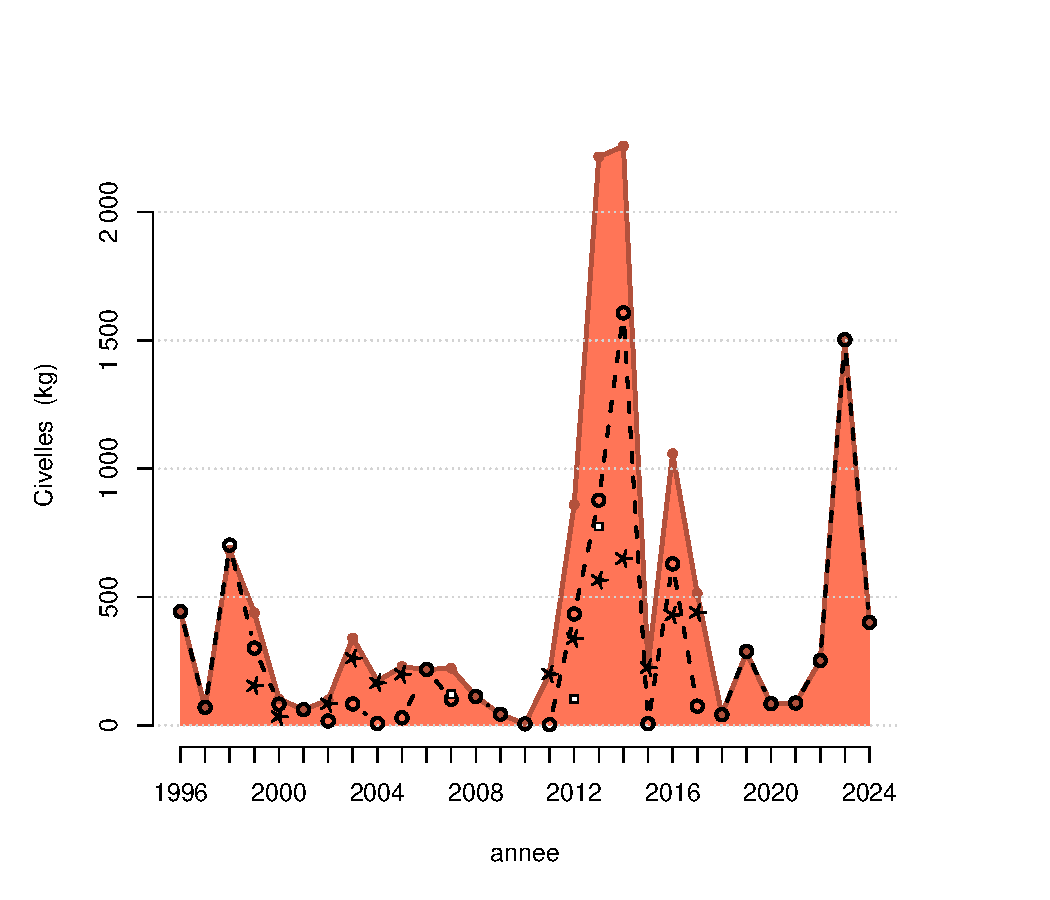
\includegraphics[width=0.5\textwidth]{figure2recrutement_kg.pdf}
\caption[Tendance des densités modèle]{Migrations de civelles (en kg)
(\textmd{{}-}o\textmd{{}-}) sur la passe au barrage d'Arzal, civelles pêchées
et transportées ($\star$) et estimation de la migration de civelles
lors des man{\oe}uvres d'écluse entre 1996 et 2011 ($\Box$). En orange, somme du
recrutement fluvial (anguilles jaunes non comprises).}
\label{figure2recrutement_kg}
\end{figure}

\subsection{Tendances de la population d'anguilles}



%
%

%

%

%

%


%




Pour l'analyse des résultats obtenus par pêche
électrique depuis 1998, seules les stations prospectées à chaque
campagne ont été conservées, soit 19 au total (9 pour le Morbihan
et 10 pour l'Ille-et-Vilaine).
%%%%%%%%%%%%%%%%%%%%%%%%%%%%%%%%%%%%%%%%%%%%%%%%%%%%%%%%%%%%%%%%%%
\small
% latex table generated in R 4.2.3 by xtable 1.8-4 package
% Wed Feb 28 11:33:39 2024
\begin{table}[htbp]
\centering
\caption[Densités et biomasses.]{Densités ($D$) et biomasses moyennes $B_e$ en anguilles (méthode Carle et Strub) et efficacités de pêche $\Phi$ calculées pour
								les 19 stations prospectées entre 1998 et 2023. Les intervalles de confiance (IC) sont
								à 0.05.} 
\label{tableau2_dens_eff_annee}
\begin{tabular}{rlrrrrrr}
  \hline
Nb & annee & $D$ & $IC~D$ & $\Phi$ & $IC~\Phi$ & $B_e$ & $IC~B_e$ \\ 
  \hline
 18 & 1998 & 0.75 & 0.38 & 0.51 & 0.07 & 16.97 & 4.46 \\ 
   19 & 1999 & 0.73 & 0.35 & 0.54 & 0.09 & 18.35 & 6.58 \\ 
   19 & 2000 & 0.88 & 0.42 & 0.59 & 0.11 & 19.10 & 5.86 \\ 
   19 & 2001 & 0.78 & 0.28 & 0.60 & 0.09 & 18.58 & 6.58 \\ 
   19 & 2002 & 0.58 & 0.29 & 0.56 & 0.12 & 13.21 & 4.65 \\ 
   19 & 2003 & 0.34 & 0.10 & 0.69 & 0.09 & 8.94 & 3.09 \\ 
   19 & 2005 & 0.23 & 0.09 & 0.75 & 0.11 & 8.08 & 3.97 \\ 
   19 & 2007 & 0.22 & 0.10 & 0.73 & 0.09 & 11.64 & 8.60 \\ 
   19 & 2009 & 0.22 & 0.08 & 0.66 & 0.12 & 8.90 & 3.43 \\ 
   19 & 2011 & 0.17 & 0.07 & 0.62 & 0.10 & 6.08 & 2.56 \\ 
   19 & 2013 & 0.28 & 0.11 & 0.57 & 0.10 & 8.90 & 4.36 \\ 
   19 & 2014 & 0.46 & 0.29 & 0.57 & 0.10 & 9.51 & 4.85 \\ 
   19 & 2015 & 0.31 & 0.13 & 0.60 & 0.11 & 5.23 & 2.29 \\ 
   19 & 2016 & 0.44 & 0.24 & 0.62 & 0.14 & 5.16 & 2.89 \\ 
   19 & 2017 & 0.21 & 0.11 & 0.56 & 0.10 & 4.83 & 2.50 \\ 
   19 & 2018 & 0.57 & 0.32 & 0.62 & 0.14 & 6.10 & 2.62 \\ 
   19 & 2019 & 0.40 & 0.21 & 0.58 & 0.13 & 5.20 & 2.41 \\ 
   19 & 2020 & 0.52 & 0.29 & 0.53 & 0.09 & 5.85 & 2.06 \\ 
   19 & 2021 & 0.41 & 0.15 & 0.64 & 0.06 & 5.58 & 1.21 \\ 
   10 & 2022 & 0.31 & 0.24 & 0.61 & 0.21 & 4.38 & 2.93 \\ 
   18 & 2023 & 0.60 & 0.30 & 0.54 & 0.08 & 6.13 & 2.13 \\ 
   \hline
\end{tabular}
\end{table}

\normalsize
%%%%%%%%%%%%%%%%%%%%%%%%%%%%%%%%%%%%%%%%%%%%%%%%%%%%%%%%%%%%%%%%%%
L'efficacité de pêche varie entre 0.51 et
0.75 (Tableau \ref{tableau2_dens_eff_annee}). 

La densité moyenne par station est
passée de 0.75 (+-0.38) anguille.m$^{-2}$ en 1998 
à 0.88 (+-0.42) anguille.m$^{-2}$ en 2000 
avant de chuter rapidement à 0.34 (+-0.1) anguille.m$^{-2}$ en 2003. 
Après un minimum de 0.17
(+-0.07) anguille.m$^{-2}$ en 2011, elle augmente
jusqu'en 2014 à 0.46
(+-0.29) anguille.m$^{-2}$
(Tableau \ref{tableau2_dens_eff_annee} et Figure \ref{dens_annee}).
Entre 2015 et 2021, elle varie entre 0.21 en
2017 et 0.57 en 2018.

%%%%%%%%%%%%%%%%%%%%%%%%%%%%%%%%%%%%%%%%%%%%%%%%%%%%%%%%%%%%%%%%%%
\begin{figure}[htbp]
\centering
 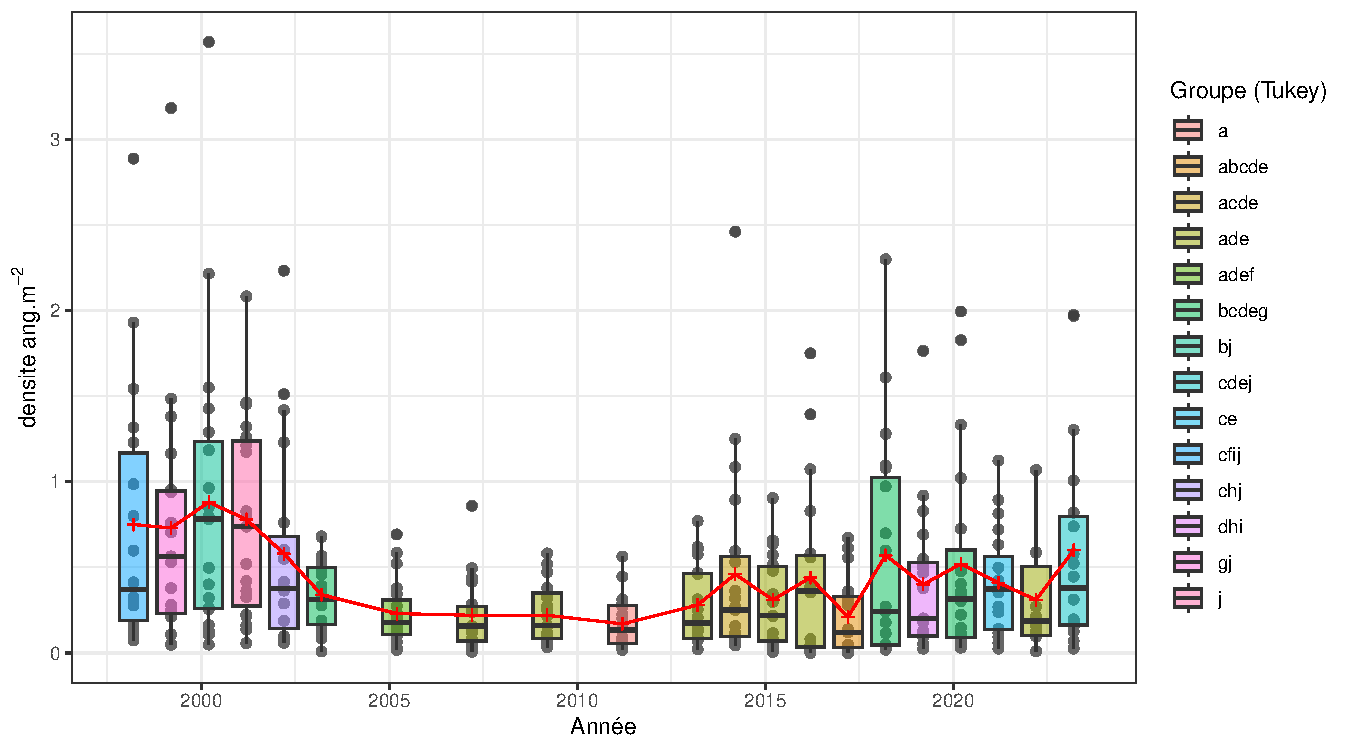
\includegraphics[width=0.5\textwidth]{dens_annee.pdf} 
\caption[Tendance des densités modèle]{Classement des densités en fonction des
années, test Post hoc de Tukey sur le modèle $log(dens) \sim a +s +
\epsilon(ss)$, avec $\epsilon(s) \sim N(0,\sigma_s^2)$ a=année, s=stations,
groupes classés au seuil de 0.05. Les moyennes du Tableau
\ref{tableau2_dens_eff_annee} sont représentées par des croix rouges.
}
\label{dens_annee}
\end{figure}
%%%%%%%%%%%%%%%%%%%%%%%%%%%%%%%%%%%%%%%%%%%%%%%%%%%%%%%%%%%%%%%%%%

L'examen des résidus du modèle glm (1) $\log
(D){\approx}a+s+m+\epsilon_s$ (modélisation des densités en fonction du mois, de
l'année et du site) montre qu'il existe une variabilité résiduelle différente en fonction des sites (Figure \ref{residus} en annexe).  Un
modèle mixte (2) incluant une variation de la dispersion des résidus en fonction
des sites $\epsilon_s=N(0,{\sigma_{s}}^2) ~s=1,\dots,19$
\citep{zuur_mixed_2009} est construit pour tenter d'homogénéiser les résidus. Le
test du rapport de vraissemblance entre les modèles mixte et le glm est
hautement significatif. Ceci indique que le modèle avec une variance différente entre
sites est meilleur et nous conduit à rejeter l'hypothèse que les variances sont
toutes égales.
La comparaison des différents modèles mixtes ((2) (3) et (4), Tableau
\ref{annex_regression_result}) montre
que le modèle incluant un effet site, un effet année et un effet mois est le
meilleur modèle car l'AIC est le plus faible (Tableau
\ref{annex_regression_result} en annexe, modèle (2)). Un modèle regroupant
uniquement les données par classes de distance \footnote{Ce modèle n'est pas présenté ici} est moins performant
qu'un modèle incluant un effet station.

Les densités ont diminué de manière
significative entre 2000 et 2003, et les années 2007 à 2013
sont significativement plus faibles que les densités de 1998 à 2003 (Tukey
Post hoc test, groupes séparés au seuil de 0.05) (Figure \ref{dens_annee},
Tableau \ref{tableau2_dens_eff_annee}).
A l'exception de l'année 2017 marquée par la sècheresse, les densités après 2014
ne sont plus différentes de celles de la période 1998-2003 et les densités moyennes sont
repassées au-dessus de la cible de gestion pour la zone à moins de 50 km de
l'estuaire avec en 2021 0.7(0.34) anguille.m$^{-2}$. Les
densités moyennes dépassent également après 2013 le seuil de 0.3
anguille.m$^{-2}$ pour la zone intérmédiaire (2021 50-100 rkm 0.31(0.25)
anguille.m$^{-2}$) et s'en approchent \footnote{Attention cependant, les deux
dernières années reflètent l'intégration des stations de la Seiche et l'abandon d'une des
stations sur le Chevré.} pour la zone amont (100-150 rkm
0.24(0.14) anguille.m$^{-2}$) (Tableau \ref{tableau3_dens_dist_annee}). 

L'évolution de la biomasse moyenne montre une variation moins marquée que celle
des densités avec des valeurs assez stables entre 1998 et 2001 avec 
16.97 (+-4.46) et
18.58 (+-6.58) g.m$^{-2}$) puis en chute de 2005 jusqu'en 2017
à 4.83  (+-2.5) g.m$^{-2}$ (Tableau \ref{tableau2_dens_eff_annee}
et Figure \ref{biom_annee}) avant une légère réaugmentation de 2018 à 2021 à
5.58  (+-1.21) g.m$^{-2}$.


\begin{figure}[htbp]
\centering
 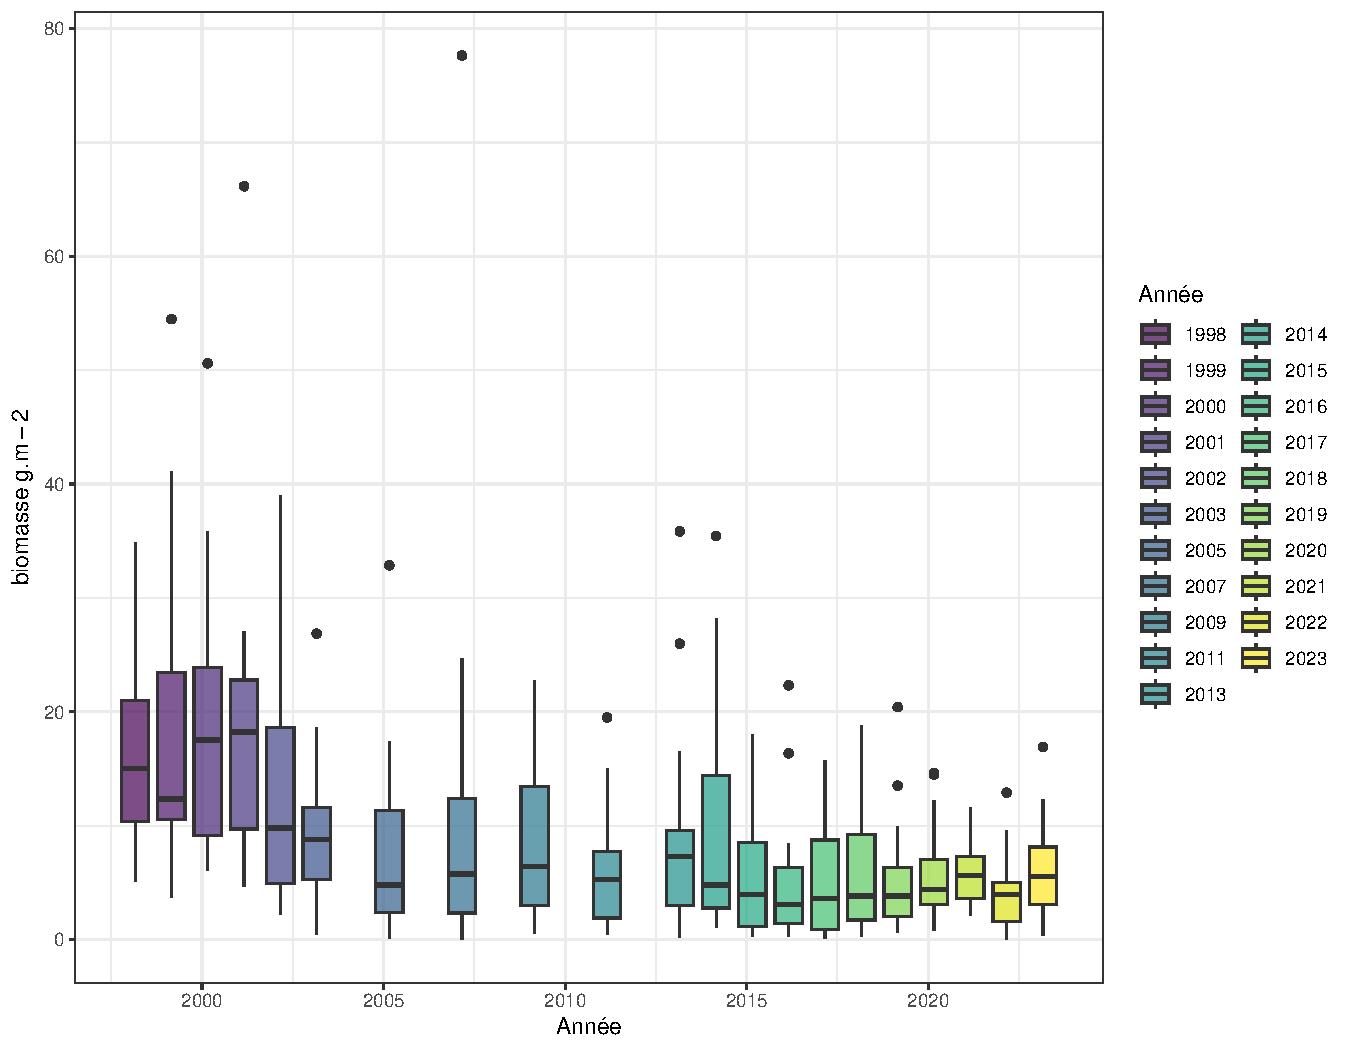
\includegraphics[width=0.5\textwidth]{biom_annee.pdf} 
\caption[Biomasses d'anguilles.]{Evolution des biomasses d'anguilles en fonction
de l'année.}
\label{biom_annee}
\end{figure}

Le déclin en densité intervient pour toutes les catégories de distance à la mer 
mais semble intervenir plus précocément
lorsqu'on se rapproche de l'estuaire (Figure \ref{dens_annee_distance},
Tableau \ref{tableau3_dens_dist_annee}).
Comme pour les densités, la chute des biomasses est
d'autant moins marquée que l'on s'éloigne du barrage d'Arzal (Figure
\ref{biom_annee_dist}, Tableau \ref{table_biom_dist_annee}).

\begin{figure}[htbp]
  \centering
    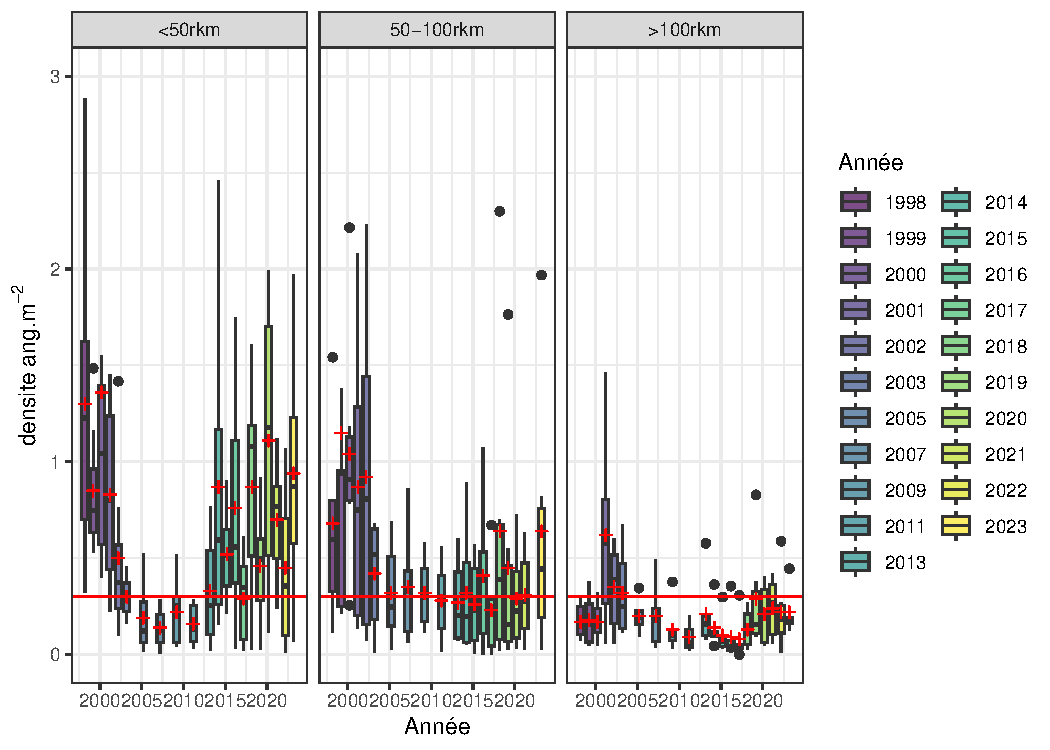
\includegraphics[width=0.5\textwidth]{dens_annee_dist.pdf}
    \caption[Densité moyennes $\sim$ distance.]{Distribution des densités
    d'anguilles par classe de distance pour les pêches
    électriques de 1998 à 2024. Les box plot représentent le premier
    et le troisième quartile, et l'axe central la médiane des densités
    d'anguilles obtenues pour les pêches de chaque année. Les barres d'erreur correspondent aux données comprises dans 1.5 fois l'écart
    interquartile. Les points au-delà représentent des "outliers" et sont
    représentés individuellement. L'axe rouge représente le seuil fixé
    actuellement dans le plan de gestion (0.3 anguille.m$^{-2}$).
     Les croix rouges correspondent aux densités
    moyennes.}
  \label{dens_annee_distance}
\end{figure} 
    
\small
% latex table generated in R 4.3.2 by xtable 1.8-4 package
% Thu Apr 10 13:13:09 2025
\begin{table}[htbp]
\centering
\caption[Densité et distance.]{Densités moyennes en anguille.m$^{-2}$ en fonction de la distance (+ - intervalles de confiance à 0.05.)} 
\label{tableau3_dens_dist_annee}
\begin{tabular}{llll}
  \hline
annee & <50rkm & 50-100rkm & >100rkm \\ 
  \hline
1998 & 1.3(0.82) & 0.68(0.68) & 0.17(0.1) \\ 
  1999 & 0.85(0.32) & 1.15(1.15) & 0.18(0.14) \\ 
  2000 & 1.36(0.99) & 1.04(0.68) & 0.17(0.11) \\ 
  2001 & 0.83(0.45) & 0.87(0.83) & 0.62(0.53) \\ 
  2002 & 0.5(0.42) & 0.92(0.92) & 0.35(0.24) \\ 
  2003 & 0.3(0.1) & 0.42(0.31) & 0.32(0.24) \\ 
  2005 & 0.19(0.17) & 0.32(0.28) & 0.2(0.09) \\ 
  2007 & 0.14(0.1) & 0.35(0.31) & 0.2(0.18) \\ 
  2009 & 0.22(0.16) & 0.32(0.19) & 0.13(0.13) \\ 
  2011 & 0.16(0.1) & 0.28(0.22) & 0.09(0.07) \\ 
  2013 & 0.33(0.27) & 0.27(0.24) & 0.21(0.2) \\ 
  2014 & 0.87(0.76) & 0.32(0.36) & 0.14(0.12) \\ 
  2015 & 0.52(0.23) & 0.26(0.25) & 0.1(0.11) \\ 
  2016 & 0.76(0.57) & 0.41(0.42) & 0.09(0.14) \\ 
  2017 & 0.29(0.22) & 0.23(0.26) & 0.08(0.12) \\ 
  2018 & 0.87(0.56) & 0.64(0.9) & 0.13(0.11) \\ 
  2019 & 0.46(0.29) & 0.45(0.7) & 0.29(0.3) \\ 
  2020 & 1.11(0.8) & 0.29(0.28) & 0.21(0.14) \\ 
  2021 & 0.7(0.34) & 0.31(0.25) & 0.24(0.14) \\ 
  2022 & 0.45(0.77) &  & 0.22(0.21) \\ 
  2023 & 0.94(0.69) & 0.64(0.75) & 0.22(0.12) \\ 
  2024 & 3.5(4.07) & 0.39(0.41) & 0.2(0.16) \\ 
   \hline
\end{tabular}
\end{table}

\normalsize

\begin{figure}[htbp]
  \centering
  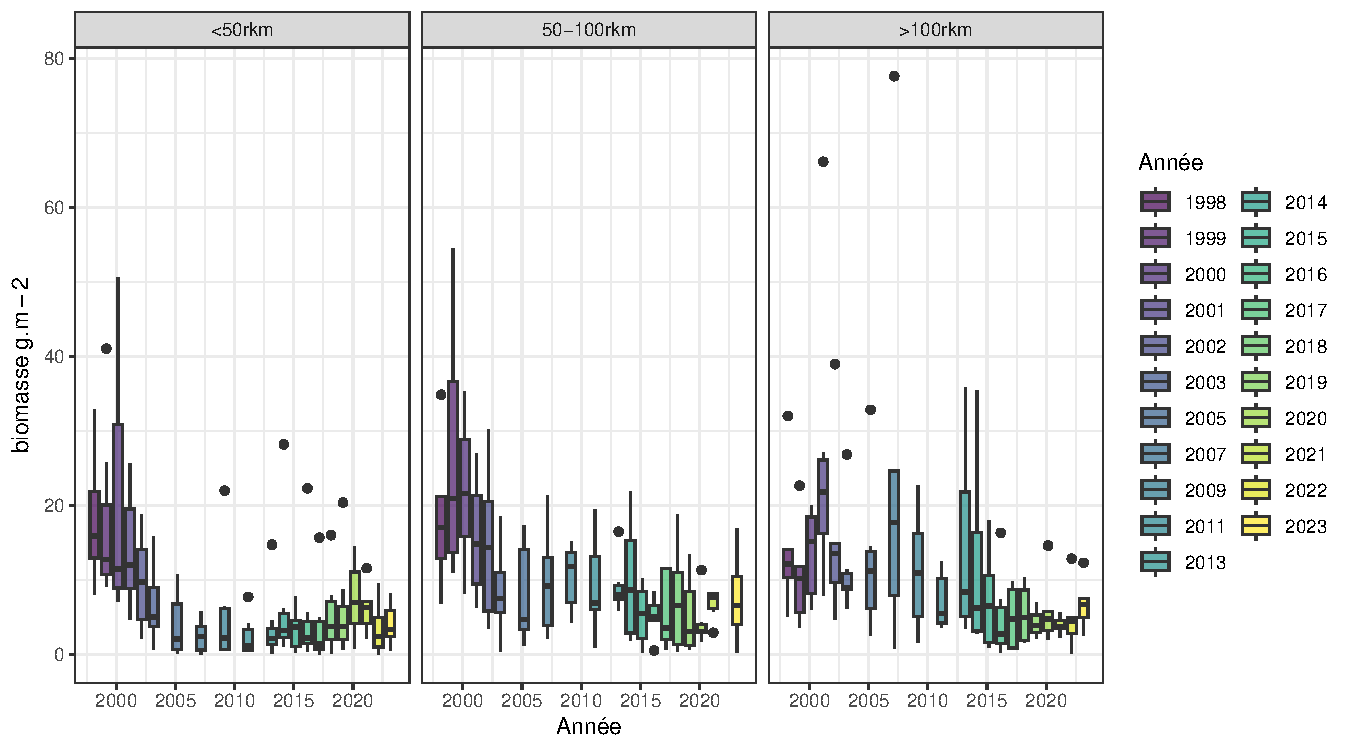
\includegraphics[width=0.5\textwidth]{biom_annee_dist.pdf}
  \caption[_court]{Biomasses moyennes d'anguilles par classe de distance pour les pêches
  électriques de 1998 à 2024. Les barres d'erreur
  correspondent aux données comprises dans 1.5 fois
  l'écart interquartile.}
  \label{biom_annee_dist}
\end{figure}

    
\small
% latex table generated in R 4.2.3 by xtable 1.8-4 package
% Fri Mar 15 14:11:21 2024
\begin{table}[htbp]
\centering
\caption[Biomasse et distance.]{Biomasses moyennes en anguilles (en g.m$^{-2}$) en fonction de la distance (+ - intervalles de confiance à 0.05).} 
\label{table_biom_dist_annee}
\begin{tabular}{llll}
  \hline
annee & <50rkm & 50-100rkm & >100rkm \\ 
  \hline
1998 & 18.1(7.83) & 18.58(13.11) & 14.32(9.73) \\ 
  1999 & 17.8(10.81) & 26.77(18.24) & 10.56(7.2) \\ 
  2000 & 21.27(15.55) & 22(10.69) & 13.66(6.43) \\ 
  2001 & 14.16(7.06) & 15.71(8.59) & 26.62(21.51) \\ 
  2002 & 9.77(6.17) & 14.69(11.03) & 15.76(12.62) \\ 
  2003 & 6.74(5.01) & 8.56(6.5) & 11.89(7.89) \\ 
  2005 & 4.01(4.34) & 8.05(7.52) & 12.87(11.3) \\ 
  2007 & 2.44(2.1) & 9.75(7.59) & 24.26(29.2) \\ 
  2009 & 5.52(7.12) & 10.48(4.75) & 11.27(8.46) \\ 
  2011 & 2.48(2.5) & 9.23(7.11) & 7.13(4.13) \\ 
  2013 & 3.85(4.62) & 9.25(3.95) & 14.42(13.98) \\ 
  2014 & 6.88(8.85) & 9.94(8.67) & 12.13(13.6) \\ 
  2015 & 3.31(2.49) & 5.35(4.24) & 7.35(7.1) \\ 
  2016 & 5.27(7.13) & 5.06(3.63) & 5.11(6.34) \\ 
  2017 & 3.95(5.09) & 5.92(6.62) & 4.99(5.27) \\ 
  2018 & 5.49(5.02) & 7.43(7.57) & 5.48(4.19) \\ 
  2019 & 6(6.35) & 5.21(5.57) & 4.25(1.93) \\ 
  2020 & 7.49(5.44) & 4.45(3.66) & 5.63(3.9) \\ 
  2021 & 6.22(3.45) & 6.8(2.23) & 3.98(0.98) \\ 
  2022 & 3.62(6.7) &  & 4.89(4.55) \\ 
  2023 & 4.08(3.01) & 7.57(6.22) & 6.76(3.48) \\ 
   \hline
\end{tabular}
\end{table}

\normalsize

Les densités d'anguilles d'âge 0 et 1 semblent remonter vers des
niveaux proches des niveaux observés au début du suivi entre 1998 et 2001. 
 (Figures \ref{dens_age_annee},
\ref{dens_age_annee_dist} en annexe, Tableau \ref{table_densite_age_annee}).
Pour les âges 2 à 4+, il y a globalement une baisse.

\begin{figure}[htbp]
\centering
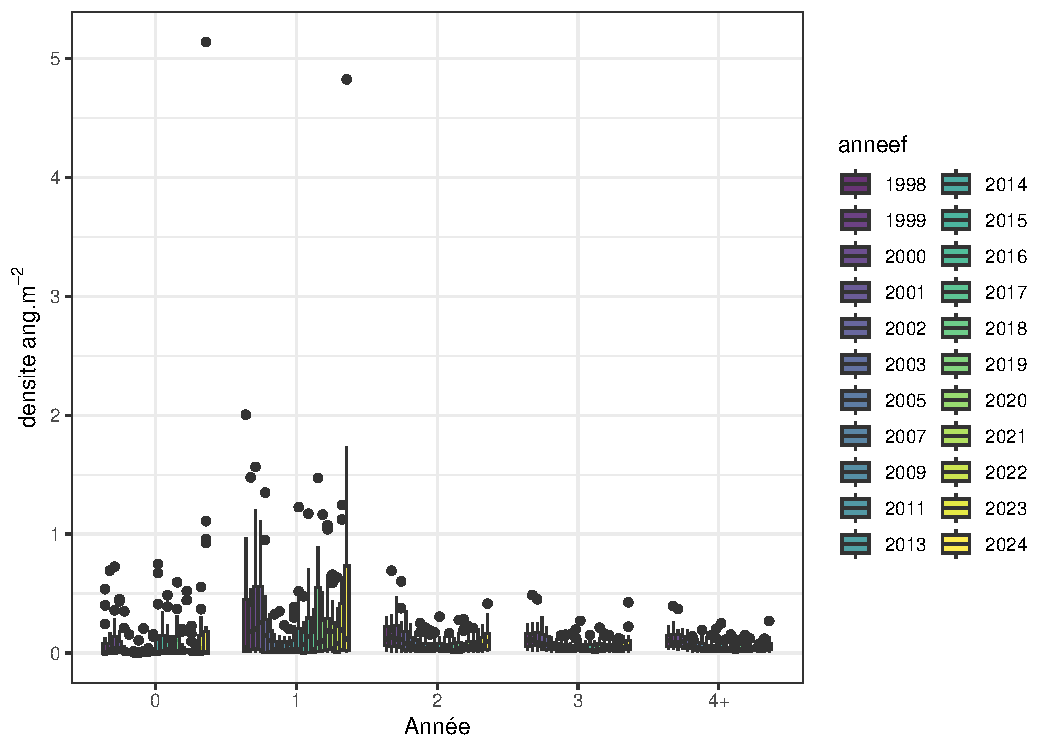
\includegraphics[width=0.5\textwidth]{dens_age_annee.pdf}
\caption[Densité par âge.]{Tendance des densités en fonction de
l'âge des anguilles (reconstituée à l'aide d'une clé taille âge) pour
les pêches électriques de 1998 à 2024 \footnotemark}.
\label{dens_age_annee}
\end{figure}

\footnotetext{Attention les
pêches électriques ont eu lieu tous les ans de 1998 à 2003, tous les
  2 ans de 2003 à 2013 avant de reprendre à une fréquence annuelle.}

La clé taille-âge utilisée doit être considérée avec précaution car il n'y a pas eu de
vérification des données de croissance.
\subsection{Marquages recaptures}


Les recaptures et marquages effectués de 2009 à 2024 sont indiqués au Tableau
\ref{tablemr}.
Les croissances des anguilles marquées sont
assez faibles avec en moyenne $20.8$ mm par an. Certaines anguilles
n'ont pas grandi du tout alors que
d'autres ont gagné 60 mm (Figures \ref{croissance} et \ref{croissance2}). En
excluant les anguilles ayant perdu du poids entre le marquage et la recapture
(18 anguilles sur
142), les croissances annuelles s'établissent à
$23.3$ mm.
%%%%%%%%%%%%%%%%%%%%%%%%%%%%%%%%%%%
% latex table generated in R 4.2.3 by xtable 1.8-4 package
% Wed Feb 28 11:33:50 2024
\begin{table}[htbp]
\centering
\caption[Marquage et recaptures. Les marques sont soit posées, soit lues lorsque l'anguille est déjà marquée.]{Marquage et recaptures.} 
\label{tablemr}
\begin{tabular}{lrr}
  \hline
 & lecture & pose \\ 
  \hline
2009 & 12 & 87 \\ 
  2011 & 21 & 63 \\ 
  2013 & 29 & 61 \\ 
  2014 & 27 & 70 \\ 
  2015 & 18 & 43 \\ 
  2016 & 16 & 38 \\ 
  2017 & 11 & 35 \\ 
  2018 & 24 & 39 \\ 
  2019 & 7 & 37 \\ 
  2020 & 10 & 38 \\ 
  2021 & 10 & 44 \\ 
  2022 & 2 & 14 \\ 
  2023 & 9 & 35 \\ 
   \hline
\end{tabular}
\end{table}

%%%%%%%%%%%%%%%%%%%%%%%%%%%%%%%%%%%
Le taux de recapture des anguilles est de
31 \%.

\begin{figure}[htbp]
\centering
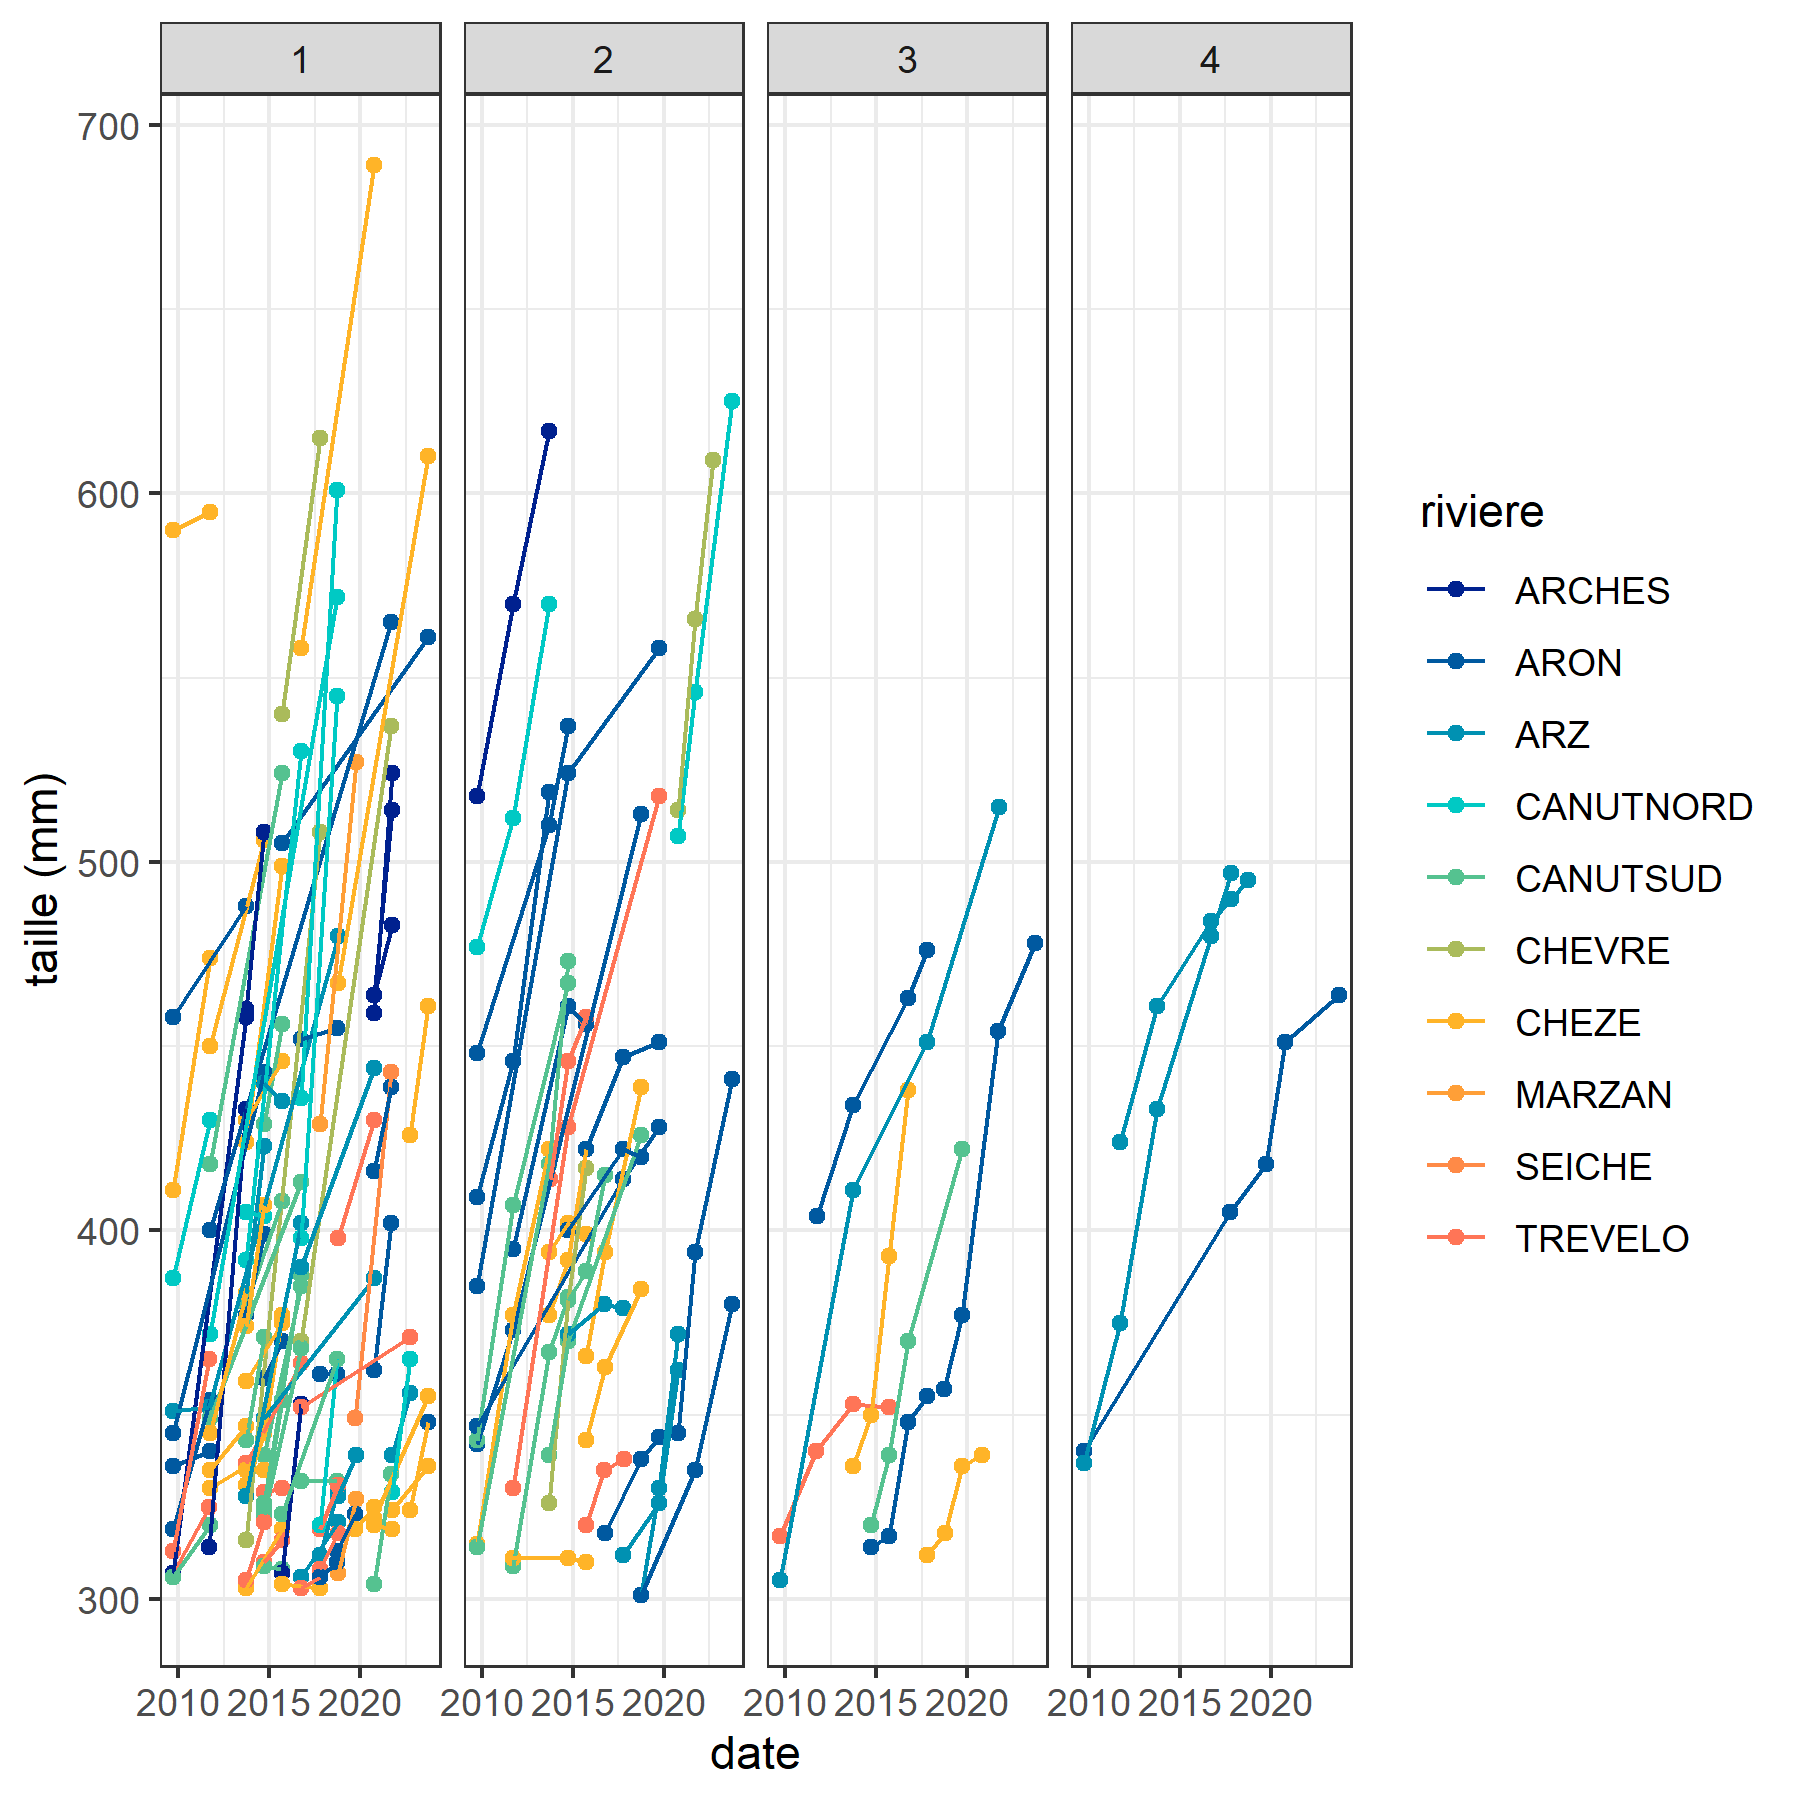
\includegraphics[width=0.5\textwidth]{croissance.png}
\caption[Taille anguilles marquées]{Evolution de la taille des anguilles
marquées, en fonction du nombre de recaptures.}
\label{croissance}
\end{figure}
Il est possible qu'un effet "marquage" apparaisse chez certaines anguilles avec
des croissances plus faibles pour certains individus lors des deux premières
années voire des pertes de poids (Figure \ref{croissance3}). Cet effet peut
être testé par l'inclusion d'une tendance non linéaire (gam) pour l'année, il
n'est pas significatif.

\begin{figure}[htbp]
\centering
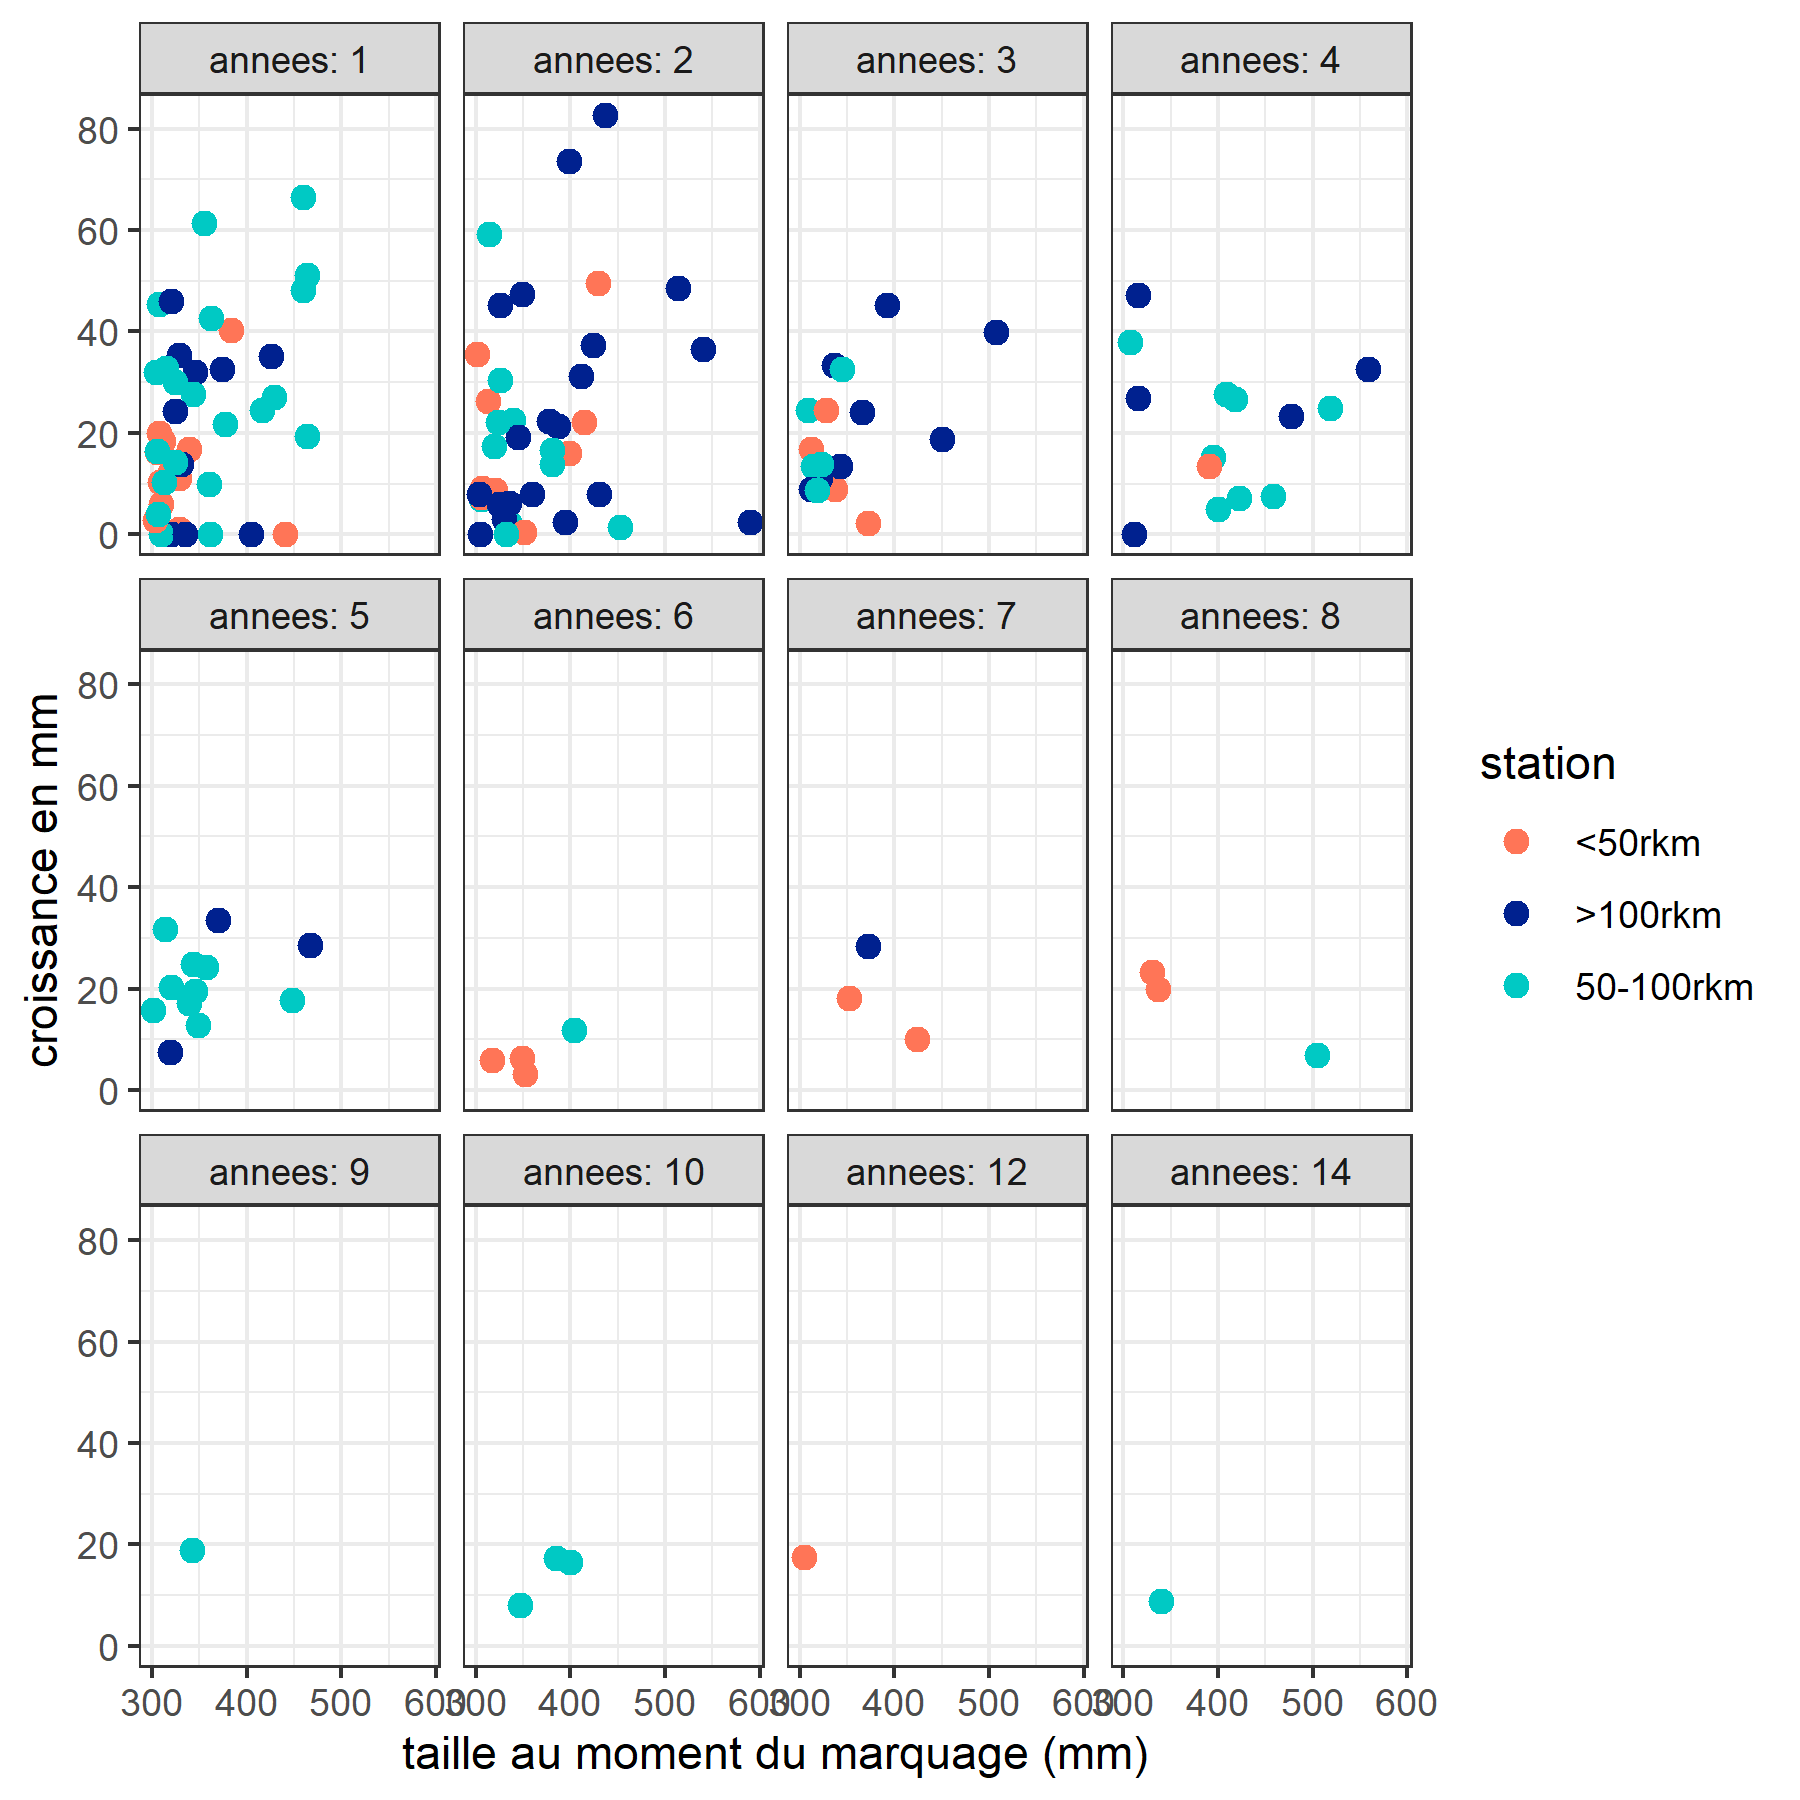
\includegraphics[width=0.5\textwidth]{croissance2.png}
\caption[Croissance annuelles des anguilles marquées]{Croissance annuelle des
anguilles marquées en fonction du nombre d'année entre le marquage et la
recapture.}
\label{croissance2}
\end{figure}


\begin{figure}[htbp]
\centering
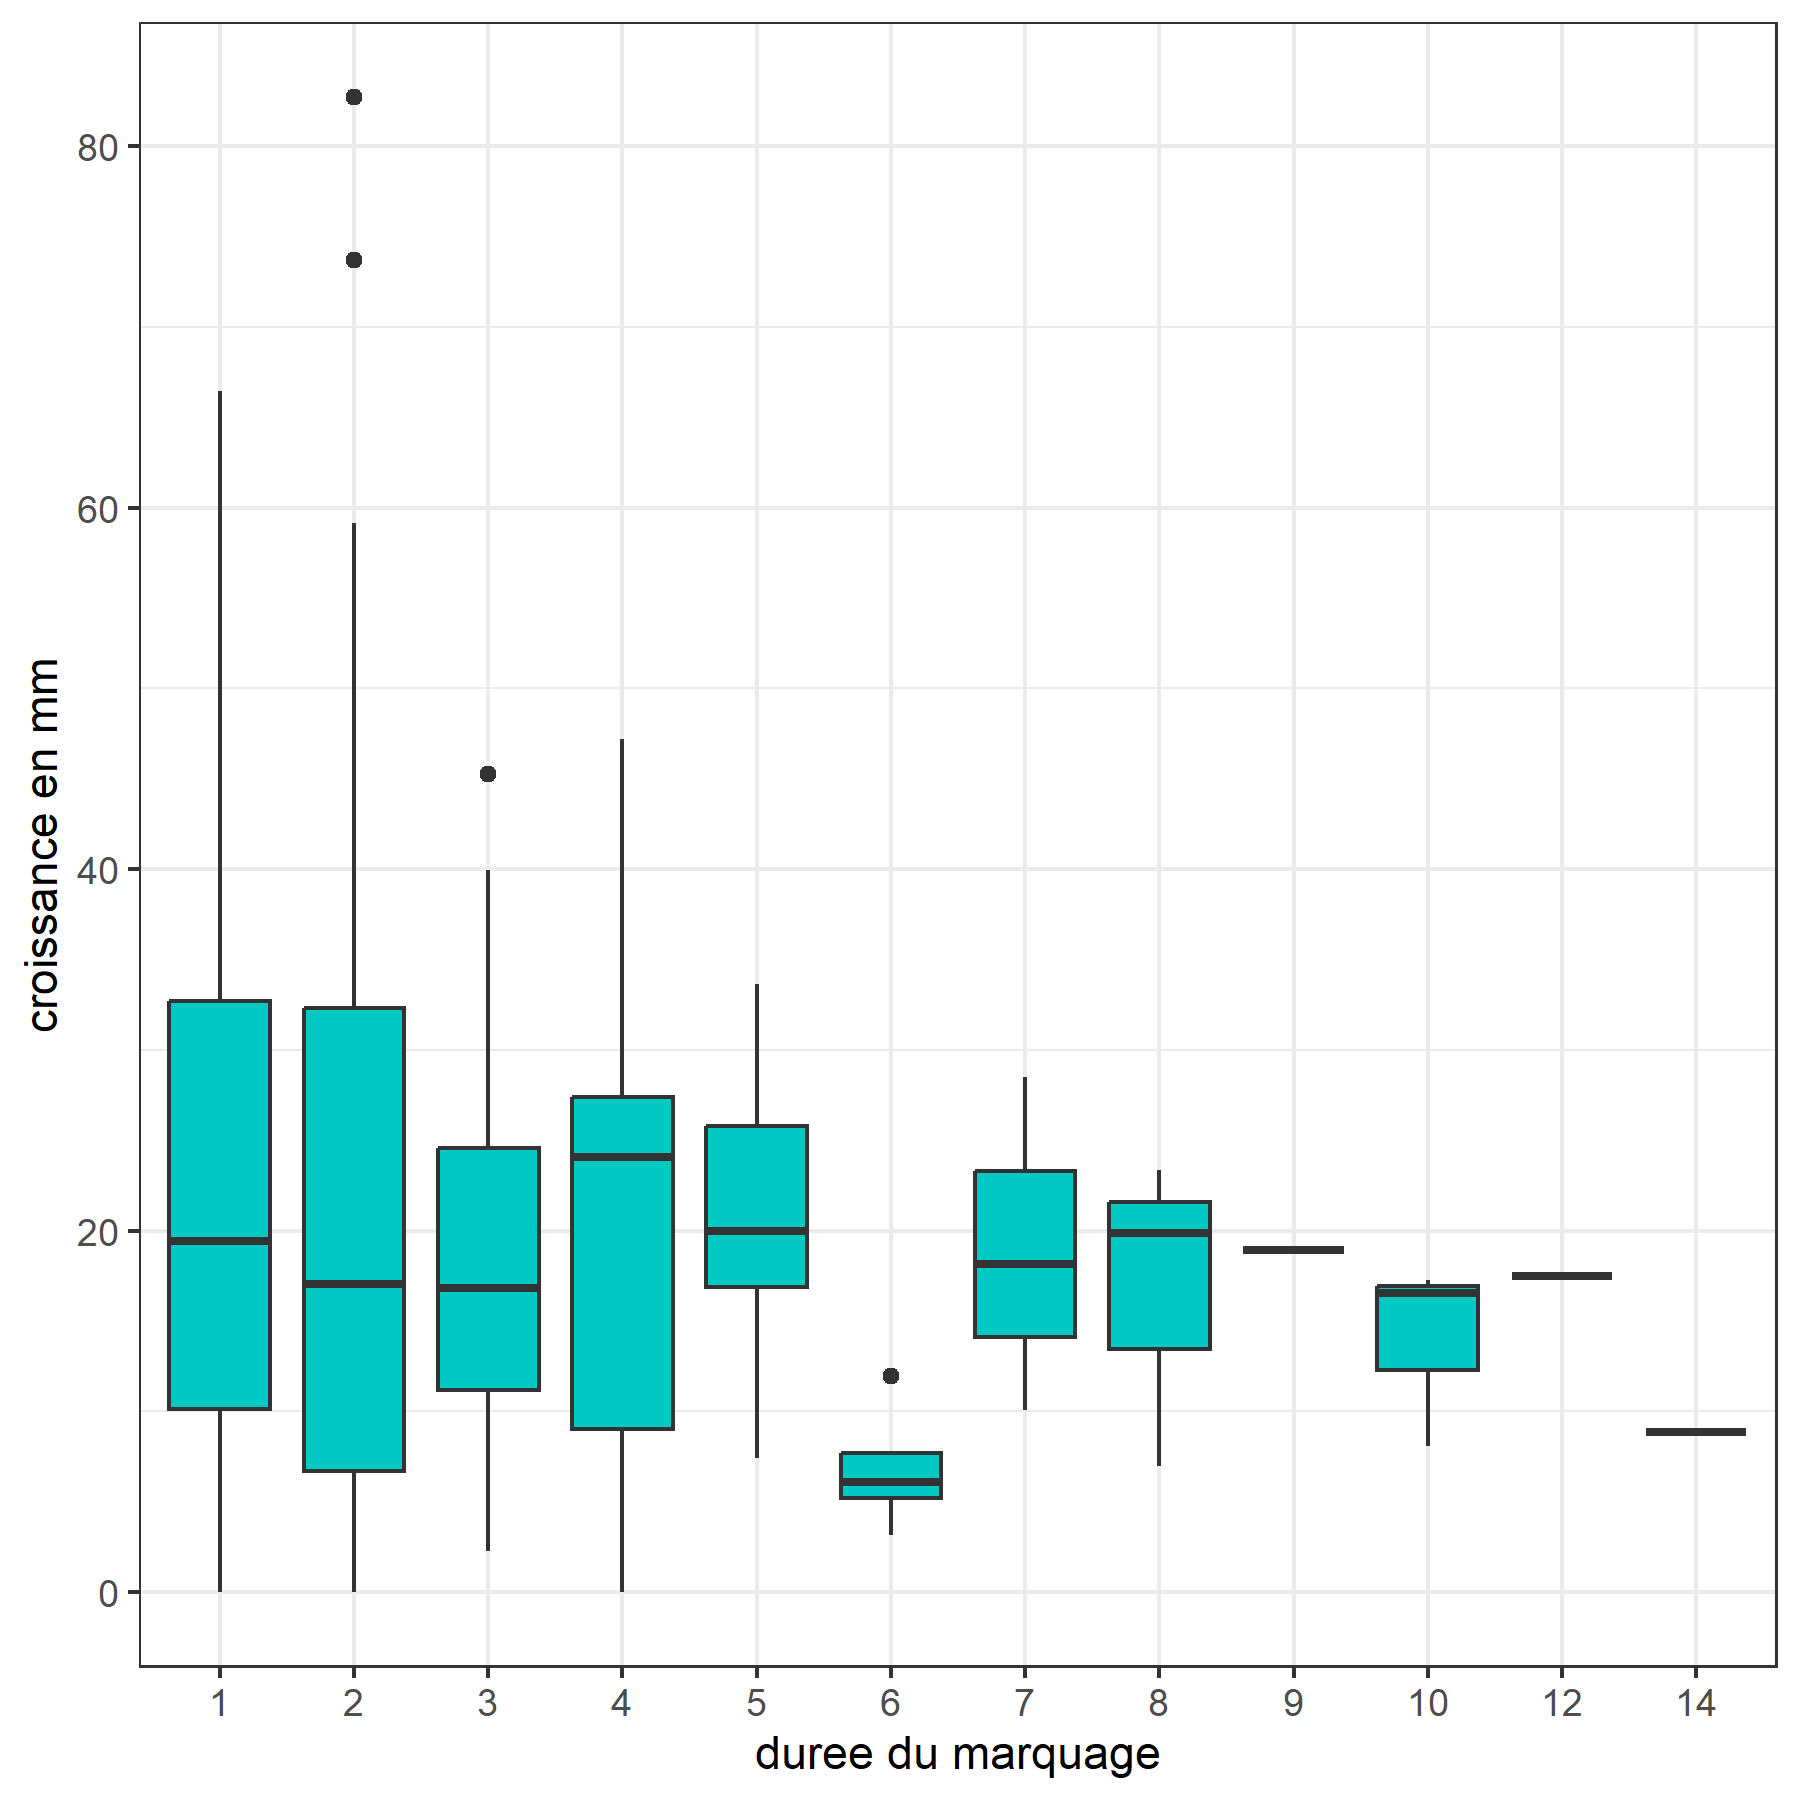
\includegraphics[width=0.5\textwidth]{croissance3.png}
\caption[Croissance annuelles des anguilles marquées]{Croissance annuelle des
anguilles marquées en fonction de la durée du marquage.}
\label{croissance3}
\end{figure}


La croissance est très variable mais il est difficile de trouver un facteur
expliquant clairement la variation observée. Il y a un effet station significatif avec des croissances plus fortes
pour certaines stations (Figure \ref{croissance4}), mais la distance n'est pas significative
quand on la teste seule. Par contre, ni le délai en années après le
marquage, ni la taille de départ au marquage, ni la zone (en grande
classe de distance) ne sont significatives dans l'analyse de variance du
modèle (Tableau \ref{table_anova_marquage}). 

% latex table generated in R 4.3.2 by xtable 1.8-4 package
% Wed Apr  9 10:37:09 2025
\begin{table}[ht]
\centering
\begin{tabular}{lrrrr}
  \hline
 & Sum Sq & Df & F values & Pr($>$F) \\ 
  \hline
station & 15616.25 & 17 & 5.40 & 0.0000 \\ 
  Residuals & 21102.46 & 124 &  &  \\ 
   \hline
\end{tabular}
\caption{Test statistique (Anova) des variables du modèle croissance annuelle $\sim$ station,
						où $station$ correspond à la station de pêche. Deux autres facteurs, année et taille au moment du marquage,
						ont été testés, ils ne sont pas significatifs.} 
\label{table_anova_marquage}
\end{table}


\begin{figure}[htbp]
\centering
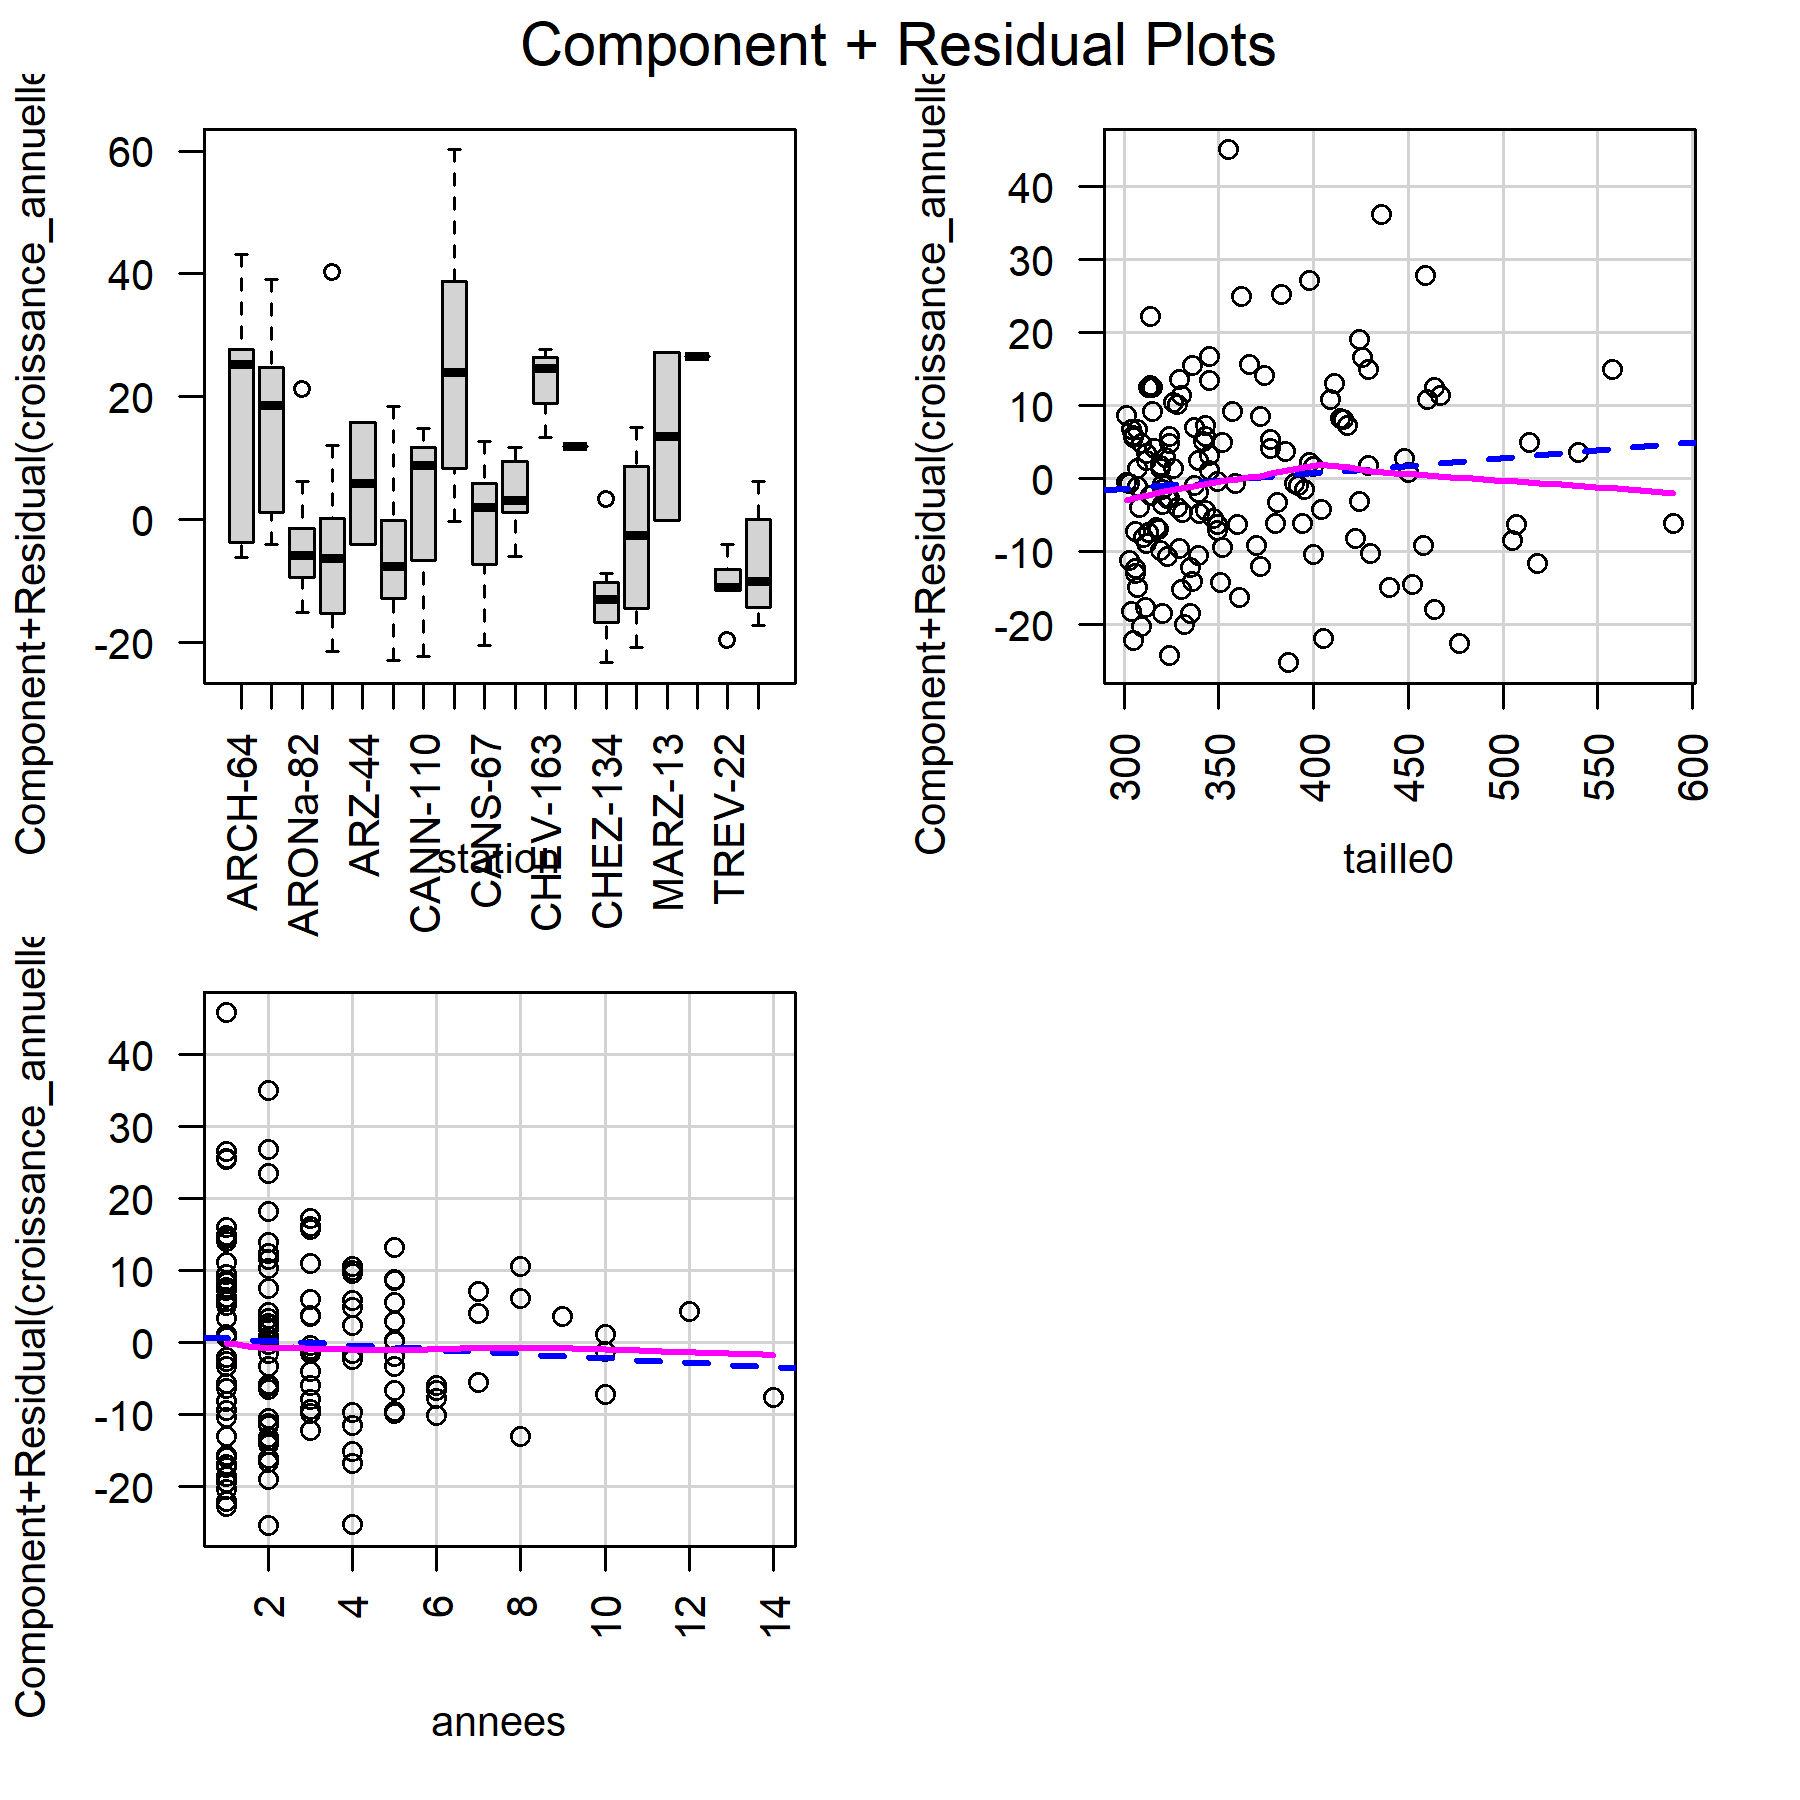
\includegraphics[width=0.5\textwidth]{croissance4.png}
\caption[Graphique de composant et résidus du modèle glm croissance ~ annee +
station + taille initiale.]{Graphique de composant et résidus (CR plot) du
modèle glm croissance ~ annee + station + taille0, où $annees$ représente le
nombre d'années entre le marquage et la recapture, $taille0$ la taille au moment
du marquage, et $station$ la station de pêche. Ce graphique indique quelle est la
moyenne des tendances (ligne rose) et l'effet ajusté (ligne bleue
pointillée).
Il permet de détecter des effets non linéaires (ici il n'y en a pas, l'écart de
la ligne rose pour les grandes tailles
(effet taille0) traduit surtout le manque de points). Il montre aussi les
résidus par station de pêche. On constate que le modèle cale des moyennes
différentes entre stations, mais aussi que la variabilité des croissances est
différente entre les stations.}
\label{croissance4}
\end{figure}


%%%%%%%%%%%%%%%%%%%%%%%%%%%%%%%%%%%%%%%%%%%%%%%%%%%%%%%%%%%%%%%%%%%%%%%%%%%%%%%%%%%%%%%
%%%%%%%%%%%%%%%%%%%%%%%%%%%%%%%%%%%%%%%%%%%%%%%%%%%%%%%%%%%%%%%%%%%%%%%%%%%%%%%%%%%%%%%
\section*{}
%\subsection{Effet du transport}

%

%%%%%%%%%%%%%%%%%%%%%%%%%%%%%%%%%%%%%%%%%%%%%%%%%%%%%%%%%%%%%%%%%%%%%%%%%%%%%%%%%%%%%%%
%%%%%%%%%%%%%%%%%%%%%%%%%%%%%%%%%%%%%%%%%%%%%%%%%%%%%%%%%%%%%%%%%%%%%%%%%%%%%%%%%%%%%%%
\section[Discussion]{ Discussion}

Les densités moyennes qui étaient passées, depuis 2005, en dessous de la cible
de 0.3 anguille.m$^{-2}$ affichée dans le plan de gestion, sont remontées
au-dessus de cette cible à partir de 2014, à l'exception de 2017 
(Figure \ref{dens_annee}, Tableau \ref{tableau2_dens_eff_annee}). 

Les biomasses d'anguilles ont par contre connu une chute
continue sur les secteurs intermédiaires et amont. Elles augmentent en aval mais
restent en deçà des valeurs observées entre 1998 et 2002 (Figures
\ref{biom_annee} et \ref{biom_annee_dist}).

Les densités de 2017 et 2019 laissent suspecter un effet de l'étiage sévère sur
certaines stations aval, où les recaptures ont été très faibles 
(ruisseau de la Bouloterie, Canut Nord et Arzal, ruisseau des
Arches proches de la rupture d'écoulement).

Les densités ont
ré-augmenté à des niveaux proches de celles de 1998 à 2012 sur la partie aval
après 2011. Elles restent plus faibles sur le secteur intermédiaire et amont
alors qu'on aurait pu s'attendre à un effet marqué des transports.
L'analyse de la fréquence en âge des captures montre bien qu'il y a eu des vagues de migration 
de jeunes anguilles, mais cette augmentation ponctuelle ne se retrouve que très
peu par la suite dans les densités d'anguilles d'âge 2 et 3 (Figure
\ref{dens_age_annee}).

Il est difficile d'expliquer les résultats obtenus. 
L'hypothèse selon laquelle il puisse y avoir un effet plus faible de la gestion 
par des effets densités dépendants est contredite par l'examen des biomasses d'anguilles
des stations qui sont bien plus faibles qu'en 1998-2002, ainsi que par les densités 
d'anguilles d'âge 2, 3 et 4 qui sont inférieures à celles de la période 1998-2000 et 
ce quels que soient les secteurs. 

Une explication possible des mauvais résultats observés peut être donnée par la
mauvaise survie de certains lots de civelles transportées, par exemple pour la
cohorte de 2011 \citep{mazel_v._operation_2011}. L'absence d'effet détectable des opérations
de transport sur les densités
observées en pêche électriques avait déjà été analysée et discutée dans
\citet{briand_analyse_2011}. Il faut également constater que la gestion par
quota a produit 4 années sur 11 entre 2009 et 2021 un
recrutement fluvial négligeable au niveau des passes d'Arzal. L'absence de
recrues pour ces années n'est probablement pas compensée par les montées importantes des autres années. 
Il est possible que de grosses vagues de migration de civelles subissent
une mortalité plus importante que des passages continus. Il est possible
également que les anguilles transportées ne se dirigent pas vers les affluents.


La croissance mesurée par pit tag est faible, de l'ordre de 20 mm par an. Comme
elle est dérivée de données de marquages pit tag, elle ne concerne que des
anguilles de taille supérieure à 30 cm.
La durée entre le marquage et la recapture n'explique pas la variation de
croissance annuelle (Figure \ref{croissance4}). La taille au moment du marquage
n'explique pas non plus la croissance. Il est difficile d'analyser les
croissances des grandes anguilles car seules quatre anguilles marquées de plus
de 50 cm ont été recapturées. 

Il est possible que les anguilles à croissance plus
rapide soient déjà parties du bassin. Les croissances moyennes calculées pour les femelles
à partir du modèle de \citet{daverat_one_2011} sont de 75, 60 et 38 mm par an pour les âges 5, 10 et 20 
\footnote{coefficients du modèle, TempSUP13=79,Ratiodistsea<-0.75}. 
Ces valeurs indiquent des croissances beaucoup plus fortes que celles trouvées sur les stations de 
la Vilaine. Cependant, les croissances annuelles calculées par le modèle de Von Bertallanffy sur
la Chèze en 1990 \citep{mounaix_intercalibration_1992} sont
seulement de 5-10 mm par an pour les anguilles de plus de 5 an. De même, les
résultats obtenus sur le Seucate (petit affluent sur le
bassin de la Dordogne) montrent que les croissances passent de 50 mm par an en
milieu fluvial large à 20 mm par an sur les
affluents (Daverat, com. pers.). 

Il existe un effet station très net dans les croissances avec des valeurs
fortes observées sur le ruisseau des Arches, le Canut Nord et le Chevré, c'est à
dire les secteurs les plus amont où les densités sont les plus faibles. Pour
autant, la prise en compte de la distance à la mer dans le modèle n'est pas
significative, car la tendance ne suit pas strictement une augmentation linéaire
des croissances en fonction de la distance.

Dans tous les cas,  on
trouve à la fois des anguilles à croissance faible et des anguilles à croissance
rapide sur les mêmes stations. Pour une anguille, une croissance négative de 5
mm a été calculée, cette anguille a également perdu beaucoup de poids. Une autre
anguille a perdu 2 mm en un an après avoir grandi les trois années précédentes.

Le fort pourcentage de recapture (31 \%) est à noter.
Il indique que les anguilles de plus de 30 cm sont globalement
sédentaires.

En utilisant les données de croissance des affluents, l'âge des anguilles est
probablement de l'ordre de 20 ans, alors qu'il ne serait que de 12 ans sur les
zones fluviales larges où la croissance est forte (de l'ordre de 50 mm par an). 

Le MNHN a analysé les otolithes de 50 anguilles argentées capturées à
Brain sur Vilaine en janvier 2016, et donne des âges compris entre 6 et 23.5
années avec une moyenne de 12 ans \footnote{Attention, ces résultats doivent être revus à la baisse avec
la ré-interprétation des stries contenues dans une bande sombre au centre de l'otolithe de certaines anguilles, mais les changements resteront marginaux.}. Les croissances mesurées varient entre 30 et 84
mm par an, soit une croissance beaucoup plus forte que celle mesurée dans les
affluents en marquage recapture. Dans le lot d'anguilles capturées, la majorité
présente des âges de 7 à 15 ans plus conforme avec la croissance de 50 mm par an
décrite par Daverat.\\ 

 \\ \mediumskip

\section[Conclusion]{Conclusion}
Les secteurs prospectés en pêche électrique, en général plutôt des petites
rivières de faible profondeur, sont caractérisés par des anguilles dont la
croissance est faible, particulièrement sur l'aval du bassin, 
alors que l'examen des anguilles capturées sur les parties aval et profonds du bassin
versant montre des anguilles de croissance plus importante, probablement ayant
des habitats de croissance différents. Sur ces affluents, après la baisse
importante du début des suivis après 1998, les transports de civelles et les
augmentations massives de recrutement sur les passes certaines années ont permis
une augmentation des densités dans les secteurs aval et les prémices d'une
augmentation sont constatés dans certains secteurs amont. 
La forte diminution du recrutement fluvial dans les 4 dernières années ne se
traduit pas par un effet notable sur les densités d'anguilles, y compris quand
on regarde la conversion en une structure en âge par des clés taille-âge.
Il est à noter que globalement, les densités sont cohérentes dans leur tendance d'une année sur 
l'autre et qu'en conséquence les tendances
obtenues sont assez crédibles, elles sont par ailleurs généralement refletées
d'un affluent à l'autre.
Il est possible que les dynamiques de croissance, colonisation et mortalité d'un
bassin saturé et de la situation "vide" d'avant l'installation des passes
engendrent des dynamiques de populations différentes, mais les biomasses, et les
densités beaucoup plus faibles d'anguilles de grande taille sur nos stations
mettent en doute cette hypothèse.
Le précédent rapport ne constatait pas d'effet des quantités importantes de
civelles ayant colonisé le bassin, grâce aux opérations de transport ou au
franchissement du barrage. Ce rapport sera plus nuancé, on perçoit des
modifications, qui ne sont pas à la hauteur attendue, et surtout qui mettent
plusieurs années pour pouvoir être observées sur les affluents. La question de
la croissance des jeunes anguilles est ici centrale et nous devrions analyser
en détail les résultats de suivi des opérations de transport qui apporteraient
ici des informations précieuses. 

\section*{Remerciements} 
Les pêches électriques ont été effectuées par les services départementaux 35 et
56 de l'OFB, nous les remercions pour leur accueil et la qualité technique de
leur travail.
Nous remercions également les différents participants qui nous ont aidé à
effectuer les pêches.
\clearpage
\onecolumn
\printbibliography
\normalsize
\clearpage
\section{Annexes}
\small

% Table created by stargazer v.5.2.3 by Marek Hlavac, Social Policy Institute. E-mail: marek.hlavac at gmail.com
% Date and time: jeu., avr. 10, 2025 - 13:01:09
\begin{table}[!htbp] \centering 
  \caption{Résultats de la régression,
				comparaison des modèles, (1) modèle linéaire $\log (D){\approx}a+s+m+\epsilon$ avec $\epsilon_s=N(0,{\sigma}^2) $
				, (2) meilleur modèle (mixte) $\log (D){\approx}a+s+m+\epsilon_s$ avec $\epsilon_s=N(0,{\sigma_{s}}^2) ~s=1,\dots,19$,
				(3) $\log (D){\approx}s+m+\epsilon_s$,
				(4) $\log (D){\approx}a+s+\epsilon_s$} 
  \label{annex_regression_result} 
\begin{tabular}{@{\extracolsep{5pt}}lcccc} 
\\[-1.8ex]\hline 
\hline \\[-1.8ex] 
 & \multicolumn{4}{c}{\textit{Dependent variable:}} \\ 
\cline{2-5} 
\\[-1.8ex] & \multicolumn{4}{c}{log(densCS)} \\ 
\\[-1.8ex] & (1) & (2) & (3) & (4)\\ 
\hline \\[-1.8ex] 
 stationARCH-66 & $-$0.158 (0.266) & $-$0.164 (0.271) & $-$0.165 (0.326) & $-$0.161 (0.270) \\ 
  stationARONa-82 & 1.341$^{***}$ (0.265) & 1.302$^{***}$ (0.244) & 1.346$^{***}$ (0.307) & 1.439$^{***}$ (0.259) \\ 
  stationARONb-82 & 1.974$^{***}$ (0.268) & 1.935$^{***}$ (0.185) & 1.932$^{***}$ (0.249) & 2.072$^{***}$ (0.200) \\ 
  stationARZ-44 & 1.879$^{***}$ (0.260) & 1.875$^{***}$ (0.290) & 1.824$^{***}$ (0.353) & 1.862$^{***}$ (0.292) \\ 
  stationARZ-47 & 2.381$^{***}$ (0.262) & 2.375$^{***}$ (0.217) & 2.350$^{***}$ (0.266) & 2.354$^{***}$ (0.225) \\ 
  stationARZA-4 & 2.415$^{***}$ (0.263) & 2.418$^{***}$ (0.221) & 2.374$^{***}$ (0.293) & 2.345$^{***}$ (0.226) \\ 
  stationCANN-110 & 0.778$^{***}$ (0.262) & 0.746$^{***}$ (0.267) & 0.749$^{**}$ (0.305) & 0.883$^{***}$ (0.277) \\ 
  stationCANN-115 & 0.802$^{***}$ (0.262) & 0.771$^{***}$ (0.240) & 0.774$^{**}$ (0.302) & 0.908$^{***}$ (0.252) \\ 
  stationCANS-67 & 1.822$^{***}$ (0.265) & 1.787$^{***}$ (0.207) & 1.819$^{***}$ (0.234) & 1.924$^{***}$ (0.207) \\ 
  stationCANSb-65 & 2.456$^{***}$ (0.265) & 2.420$^{***}$ (0.201) & 2.452$^{***}$ (0.266) & 2.557$^{***}$ (0.210) \\ 
  stationCHEV-163 & 0.152 (0.263) & 0.129 (0.222) & 0.117 (0.268) & 0.210 (0.245) \\ 
  stationCHEVa-165 & 0.181 (0.284) & 0.121 (0.227) & 0.125 (0.266) & 0.208 (0.249) \\ 
  stationCHEZ-134 & $-$0.013 (0.264) & $-$0.030 (0.234) & $-$0.020 (0.280) & 0.082 (0.236) \\ 
  stationCHEZa-135 & 1.453$^{***}$ (0.261) & 1.426$^{***}$ (0.200) & 1.421$^{***}$ (0.243) & 1.538$^{***}$ (0.210) \\ 
  stationMARZ-13 & 0.472$^{*}$ (0.278) & 0.439$^{*}$ (0.234) & 0.392 (0.316) & 0.403 (0.260) \\ 
  stationSEICH-149 & 0.101 (0.531) & 0.211 (0.187) & 0.146 (0.217) & 0.290 (0.225) \\ 
  stationSEICH-150 & 1.280$^{***}$ (0.399) & 1.356$^{***}$ (0.501) & 1.291$^{***}$ (0.484) & 1.445$^{***}$ (0.515) \\ 
  stationTREV-22 & 1.192$^{***}$ (0.260) & 1.193$^{***}$ (0.285) & 1.133$^{***}$ (0.351) & 1.155$^{***}$ (0.289) \\ 
  stationTREV-bou & 1.458$^{***}$ (0.260) & 1.454$^{***}$ (0.366) & 1.403$^{***}$ (0.409) & 1.441$^{***}$ (0.372) \\ 
  stationTREV-pes & 2.115$^{***}$ (0.260) & 2.116$^{***}$ (0.258) & 2.056$^{***}$ (0.304) & 2.078$^{***}$ (0.267) \\ 
  annee1999 & 0.149 (0.280) & 0.326 (0.221) &  & 0.153 (0.225) \\ 
  annee2000 & 0.187 (0.277) & 0.257 (0.229) &  & 0.246 (0.233) \\ 
  annee2001 & 0.330 (0.280) & 0.439$^{**}$ (0.219) &  & 0.269 (0.225) \\ 
  annee2002 & $-$0.103 (0.280) & 0.116 (0.219) &  & $-$0.057 (0.225) \\ 
  annee2003 & $-$0.436 (0.280) & $-$0.371$^{*}$ (0.219) &  & $-$0.509$^{**}$ (0.225) \\ 
  annee2005 & $-$0.872$^{***}$ (0.280) & $-$0.652$^{***}$ (0.219) &  & $-$0.828$^{***}$ (0.225) \\ 
  annee2007 & $-$1.244$^{***}$ (0.277) & $-$0.903$^{***}$ (0.218) &  & $-$0.851$^{***}$ (0.225) \\ 
  annee2009 & $-$1.093$^{***}$ (0.277) & $-$0.835$^{***}$ (0.218) &  & $-$0.786$^{***}$ (0.225) \\ 
  annee2011 & $-$1.449$^{***}$ (0.277) & $-$1.209$^{***}$ (0.218) &  & $-$1.127$^{***}$ (0.225) \\ 
  annee2013 & $-$0.951$^{***}$ (0.277) & $-$0.728$^{***}$ (0.218) &  & $-$0.664$^{***}$ (0.225) \\ 
  annee2014 & $-$0.700$^{**}$ (0.277) & $-$0.608$^{***}$ (0.218) &  & $-$0.520$^{**}$ (0.225) \\ 
  annee2015 & $-$1.041$^{***}$ (0.277) & $-$0.891$^{***}$ (0.218) &  & $-$0.833$^{***}$ (0.225) \\ 
  annee2016 & $-$0.999$^{***}$ (0.281) & $-$0.789$^{***}$ (0.220) &  & $-$0.722$^{***}$ (0.227) \\ 
  annee2017 & $-$1.053$^{***}$ (0.310) & $-$0.606$^{**}$ (0.248) &  & $-$1.148$^{***}$ (0.231) \\ 
  annee2018 & $-$0.573$^{**}$ (0.280) & $-$0.420$^{*}$ (0.219) &  & $-$0.506$^{**}$ (0.225) \\ 
  annee2019 & $-$0.662$^{**}$ (0.280) & $-$0.541$^{***}$ (0.182) &  & $-$0.620$^{***}$ (0.212) \\ 
  annee2020 & $-$0.269 (0.294) & $-$0.337 (0.214) &  & $-$0.695$^{***}$ (0.212) \\ 
  annee2021 & $-$0.571$^{**}$ (0.279) & $-$0.531$^{***}$ (0.182) &  & $-$0.502$^{**}$ (0.212) \\ 
  annee2022 & $-$1.118$^{***}$ (0.336) & $-$1.057$^{***}$ (0.311) &  & $-$1.077$^{***}$ (0.317) \\ 
  annee2023 & $-$0.434 (0.282) & $-$0.268 (0.224) &  & $-$0.237 (0.230) \\ 
  annee2024 & $-$0.256 (0.282) & $-$0.288 (0.224) &  & $-$0.210 (0.230) \\ 
  mois2oct\_nov & $-$0.449$^{***}$ (0.147) & $-$0.551$^{***}$ (0.124) & $-$0.351$^{***}$ (0.009) &  \\ 
  Constant & $-$1.930$^{***}$ (0.271) & $-$2.037$^{***}$ (0.226) & $-$2.509$^{***}$ (0.217) & $-$2.164$^{***}$ (0.237) \\ 
 \hline \\[-1.8ex] 
Observations & 403 & 403 & 403 & 403 \\ 
Log Likelihood & $-$508.335 & $-$468.846 & $-$508.807 & $-$475.631 \\ 
Akaike Inf. Crit. & 1,104.670 & 1,065.691 & 1,103.615 & 1,077.261 \\ 
Bayesian Inf. Crit. & 1,275.659 & 1,314.402 & 1,273.155 & 1,322.261 \\ 
\hline 
\hline \\[-1.8ex] 
\textit{Note:}  & \multicolumn{4}{r}{$^{*}$p$<$0.1; $^{**}$p$<$0.05; $^{***}$p$<$0.01} \\ 
\end{tabular} 
\end{table} 

\normalsize
%\begin{figure}[htbp]
%\centering
%\includegraphics[width=0.8\textwidth]{2021/densiteannuelle.pdf}
%\caption[Tendance des densités modèle]{Classement des densités en fonction des
%années, test Post hoc de Tukey sur le modèle $log(dens) \sim a +s +
%\epsilon(ss)$, avec $\epsilon(s) \sim N(0,\sigma_s^2)$ a=année, s=stations,
%groupes classés au seuil de 0.05, données log transformées.}
%\label{densiteannuelle}
%\end{figure}
%%%%%%%%%%%%%%%%%%%%%%%%%%%%%%%%%%%%%%%%%%%%%%%%%%%%%%%%%%%
\begin{figure}[htbp]
\centering
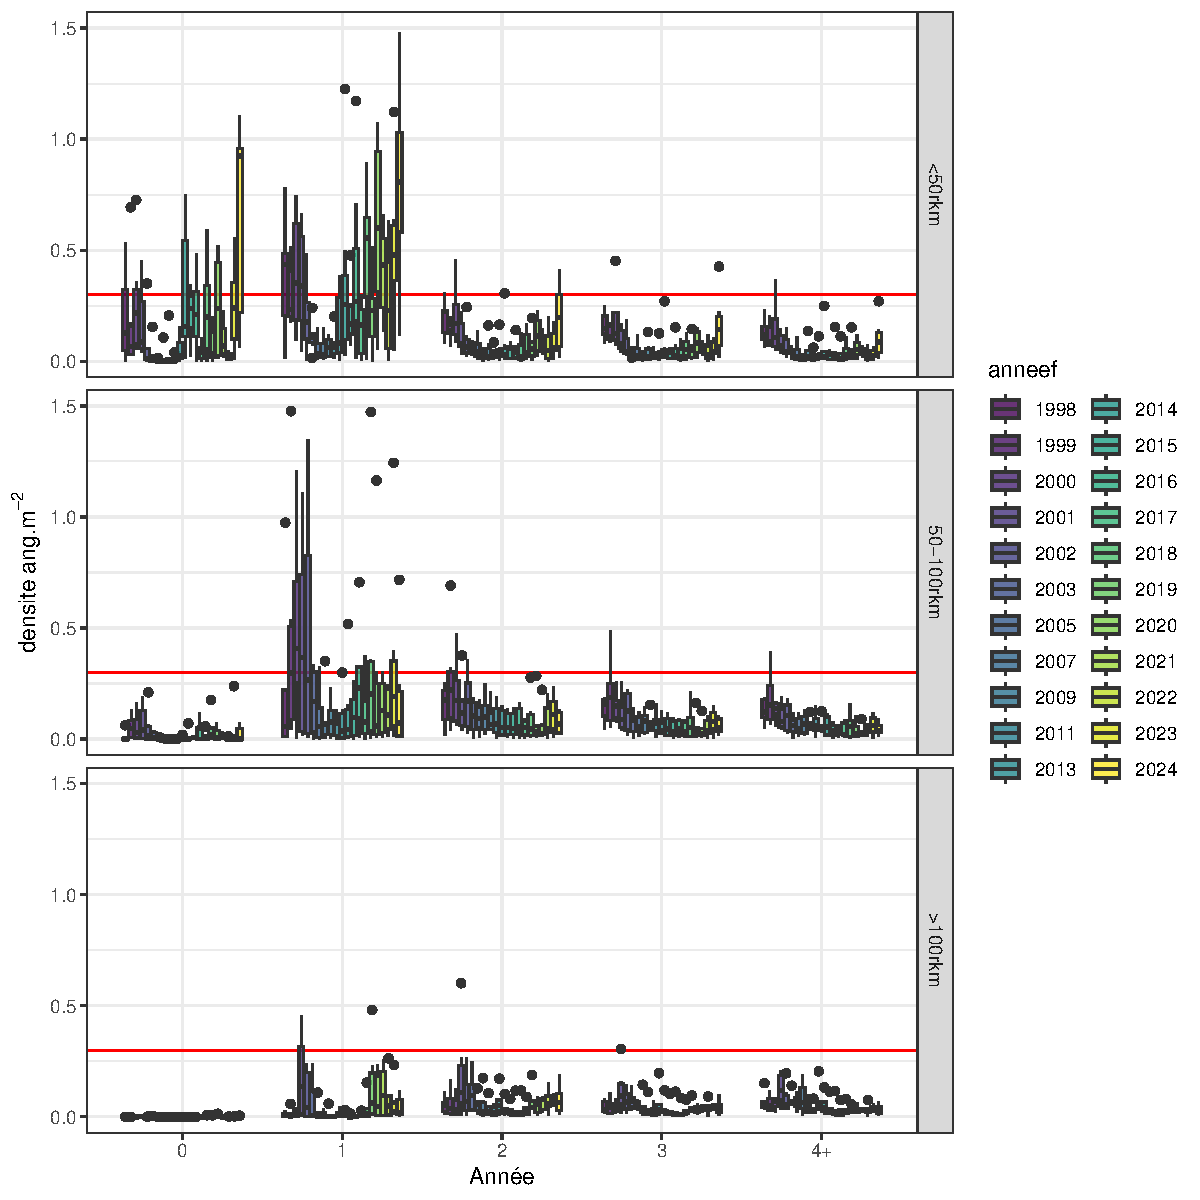
\includegraphics[width=0.8\textwidth]{dens_age_annee_dist.pdf}
\caption[Densité par âge et distance.]{Tendance des
densités en fonction de l'âge des anguilles (reconstituée à l'aide d'une clé
taille âge) et la distance à la mer pour les pêches électriques de 1998 à 2024.
La courbe en rouge indique le seuil du plan de gestion.}
\label{dens_age_annee_dist}
\end{figure}
%%%%%%%%%%%%%%%%%%%%%%%%%%%%%%%%%%%%%%%%%%%%%%%%%%%%%%%%%%%
% latex table generated in R 4.3.2 by xtable 1.8-4 package
% Thu Apr 10 13:13:12 2025
\begin{table}[htbp]
\centering
\caption[Densité âge et distance.]{Densité moyennes en anguilles (en anguille.m$^{-2}$) en fonction de la distance à la mer et de l'âge + - intervalles de confiance à 0.05.} 
\label{table_densite_age_annee}
\begin{tabular}{llllll}
  \hline
annee & 0 & 1 & 2 & 3 & 4+ \\ 
  \hline
1998 & 0.08(0.08) & 0.31(0.26) & 0.13(0.05) & 0.11(0.04) & 0.11(0.03) \\ 
  1999 & 0.08(0.08) & 0.26(0.17) & 0.15(0.07) & 0.13(0.05) & 0.12(0.04) \\ 
  2000 & 0.11(0.09) & 0.37(0.22) & 0.16(0.07) & 0.13(0.05) & 0.12(0.04) \\ 
  2001 & 0.09(0.07) & 0.33(0.16) & 0.15(0.07) & 0.11(0.04) & 0.1(0.03) \\ 
  2002 & 0.04(0.04) & 0.25(0.17) & 0.12(0.05) & 0.09(0.03) & 0.08(0.03) \\ 
  2003 & 0.02(0.02) & 0.12(0.05) & 0.09(0.03) & 0.06(0.02) & 0.06(0.02) \\ 
  2005 & 0(0) & 0.06(0.04) & 0.07(0.03) & 0.05(0.02) & 0.05(0.02) \\ 
  2007 & 0.01(0.01) & 0.05(0.04) & 0.06(0.03) & 0.05(0.02) & 0.05(0.03) \\ 
  2009 & 0.01(0.02) & 0.05(0.03) & 0.06(0.03) & 0.05(0.02) & 0.05(0.02) \\ 
  2011 & 0(0) & 0.05(0.03) & 0.05(0.02) & 0.04(0.02) & 0.04(0.02) \\ 
  2013 & 0.02(0.02) & 0.09(0.06) & 0.06(0.03) & 0.05(0.02) & 0.05(0.02) \\ 
  2014 & 0.12(0.11) & 0.17(0.15) & 0.06(0.03) & 0.05(0.03) & 0.06(0.03) \\ 
  2015 & 0.08(0.06) & 0.11(0.06) & 0.05(0.02) & 0.04(0.02) & 0.03(0.01) \\ 
  2016 & 0.1(0.07) & 0.23(0.16) & 0.05(0.03) & 0.04(0.02) & 0.04(0.02) \\ 
  2017 & 0.02(0.02) & 0.1(0.06) & 0.04(0.02) & 0.03(0.02) & 0.03(0.02) \\ 
  2018 & 0.1(0.08) & 0.31(0.19) & 0.06(0.04) & 0.05(0.03) & 0.04(0.02) \\ 
  2019 & 0.04(0.03) & 0.21(0.14) & 0.07(0.04) & 0.05(0.02) & 0.04(0.02) \\ 
  2020 & 0.08(0.08) & 0.27(0.16) & 0.07(0.03) & 0.05(0.02) & 0.04(0.02) \\ 
  2021 & 0.03(0.03) & 0.21(0.09) & 0.08(0.03) & 0.05(0.01) & 0.04(0.01) \\ 
  2022 & 0.01(0.01) & 0.16(0.15) & 0.07(0.05) & 0.04(0.03) & 0.03(0.02) \\ 
  2023 & 0.1(0.08) & 0.31(0.19) & 0.09(0.03) & 0.06(0.02) & 0.05(0.02) \\ 
  2024 & 0.48(0.61) & 0.62(0.58) & 0.12(0.06) & 0.09(0.05) & 0.06(0.03) \\ 
   \hline
\end{tabular}
\end{table}


\begin{figure}[htbp]
\centering
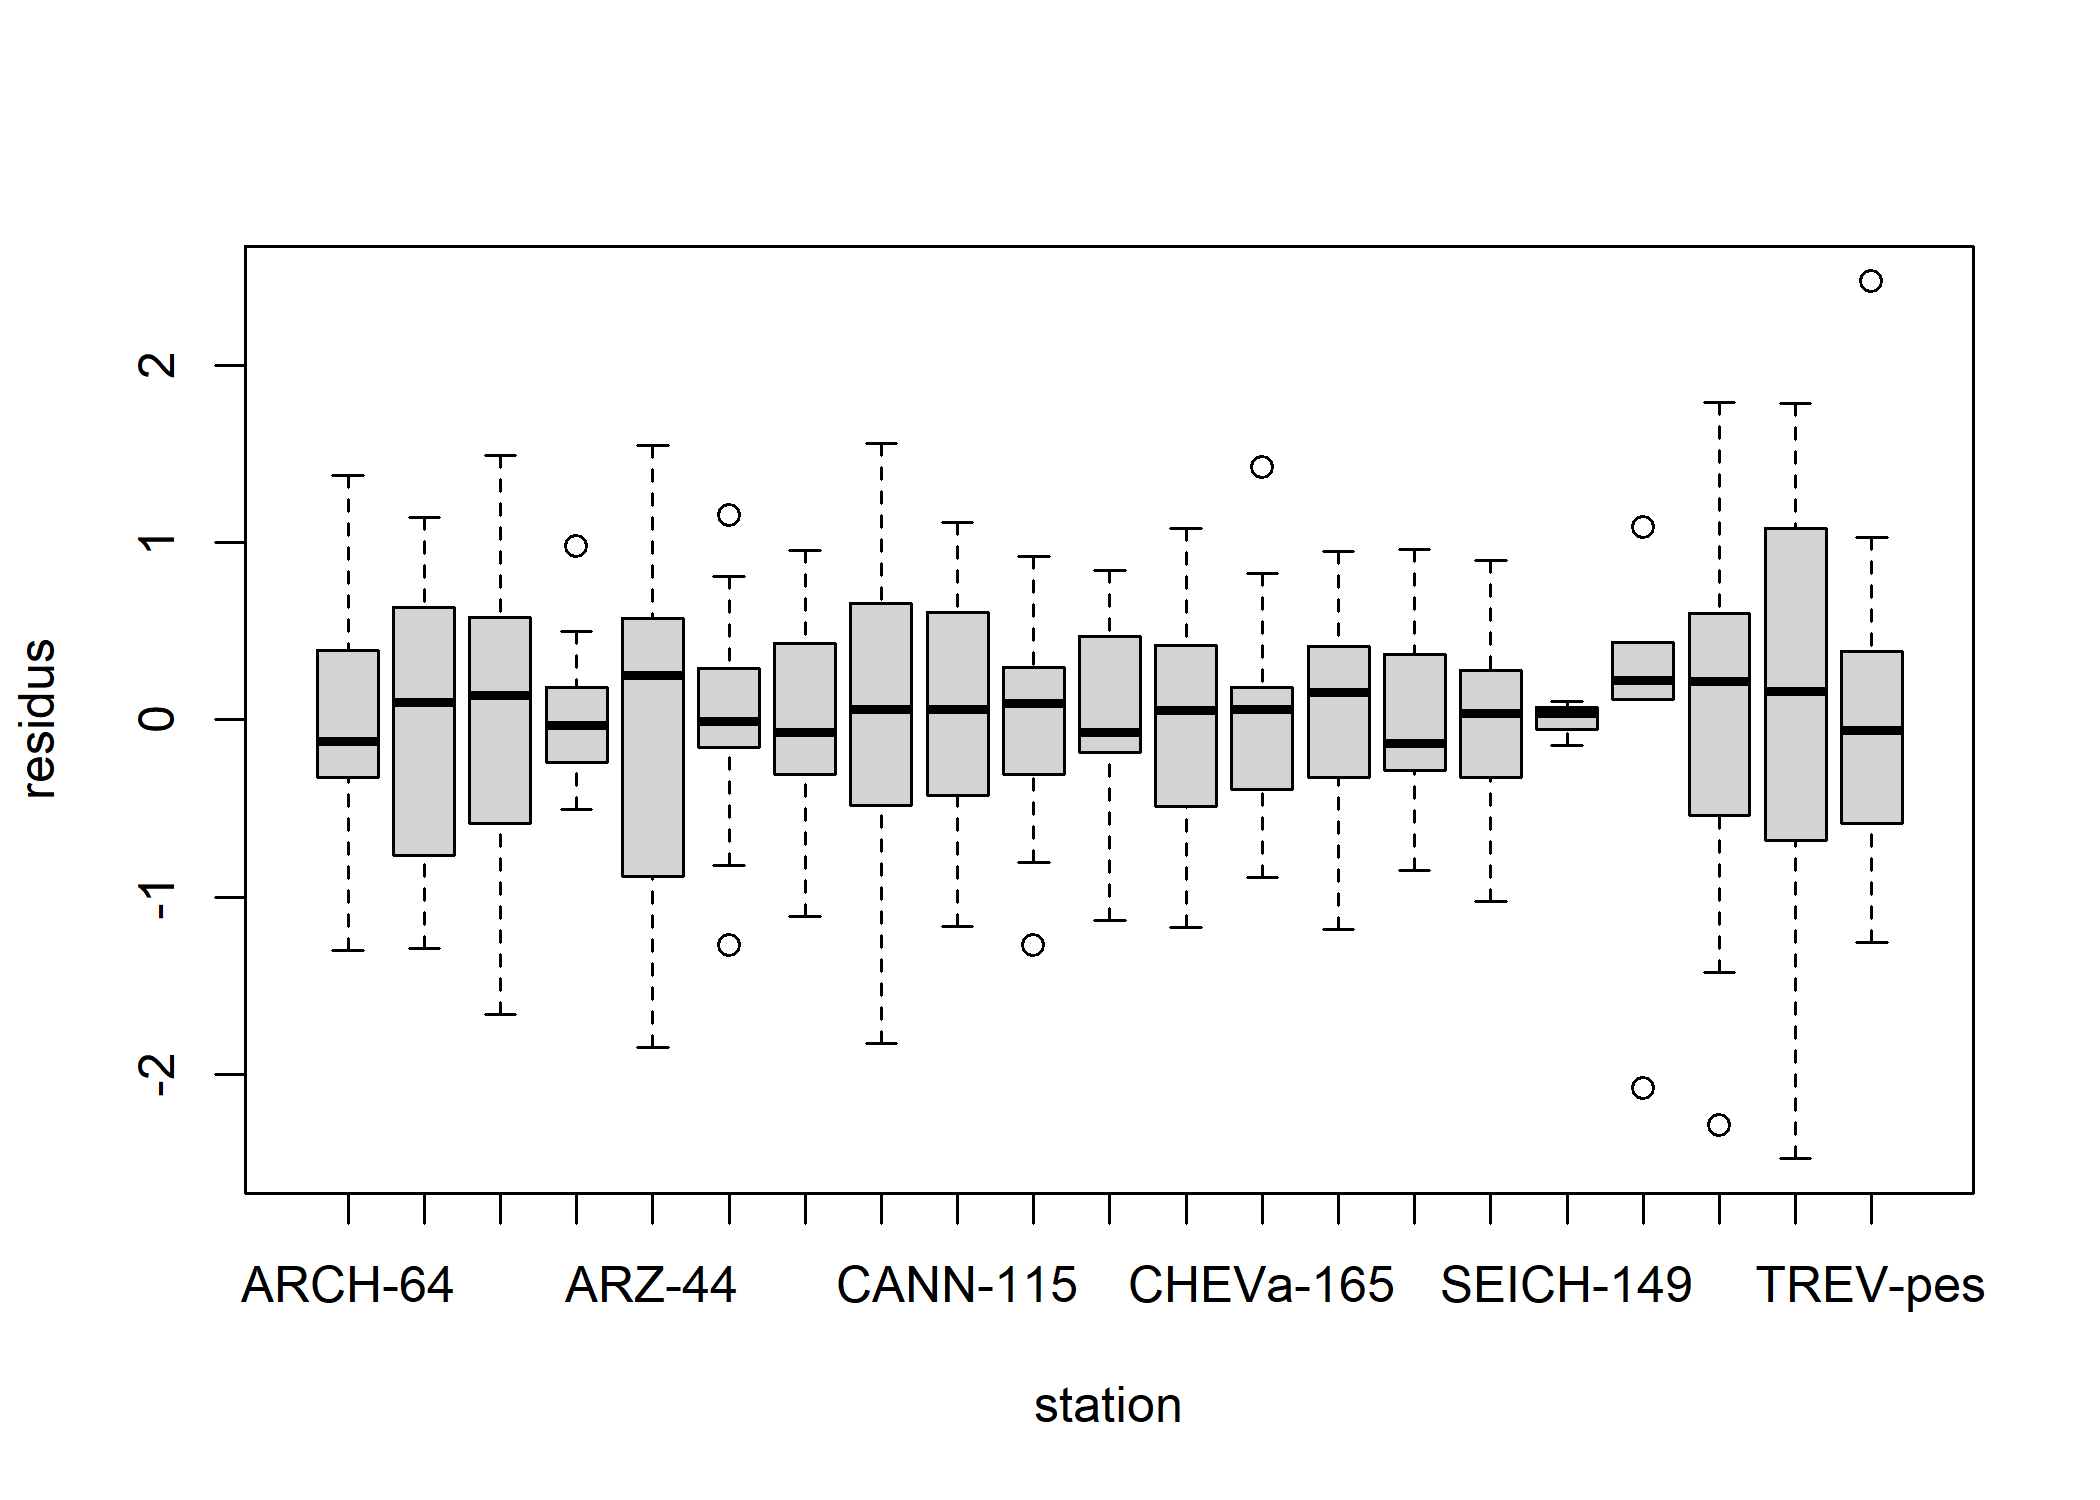
\includegraphics[width=0.8\textwidth]{residus.png}
\caption[Tendance des densités modèle]{Résidus du modèle $log(dens) \sim a +s +m
\epsilon$, avec $\epsilon(s) \sim N(0,\sigma^2)$ a=année, s=stations, m = mois.
Le graphique montre l'hétérodasticité (variances différentes) des résidus en
fonction des stations.}
\label{residus}
\end{figure}

\begin{figure}[htbp]
\centering
 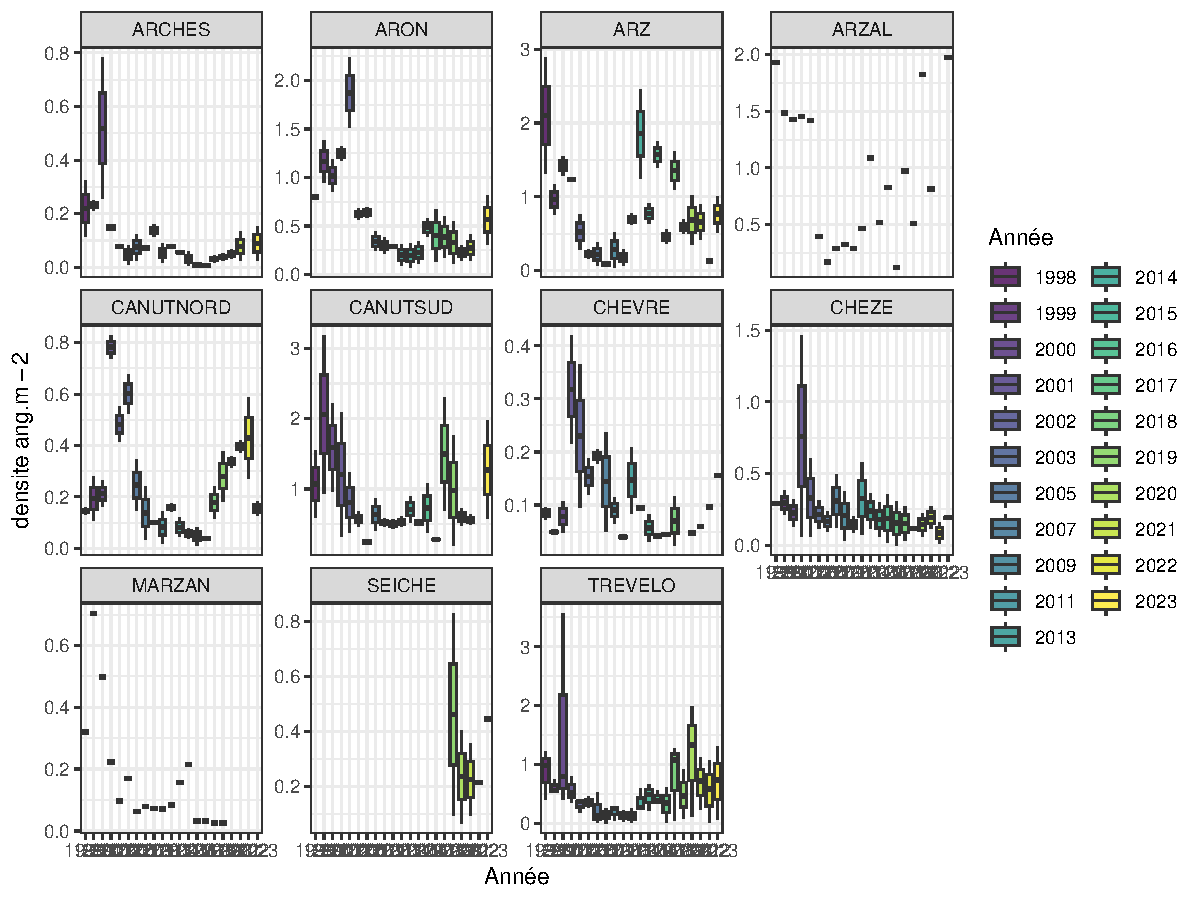
\includegraphics[width=0.8\textwidth]{dens_annee_riviere}
\caption[Tendance des densités par rivières]{Tendance des densités sur les
différents affluants du bassin versant de la Vilaine.}
\label{dens_annee_riviere}
\end{figure}

% cette figure est copiée depuis le rapport anguille voir
% C:\workspace\rapport_anguille\image\2024\recrutement_vilaine_europeen.png
\begin{figure}[htpb]
\centering
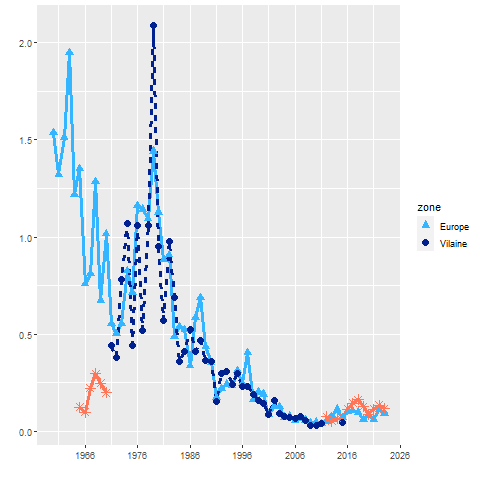
\includegraphics[width=0.8\textwidth]{../recrutement_vilaine_europeen.png}
\caption{Indice de recrutement européen du WGEEL: moyenne géométrique des
prédiction de recrutement (GLM) pour tous les sites en dehors de la mer du nord
jusqu'à 2024. Le modèle GLM ($recruit \sim area:year+site$) est calé sur
les séries de recrutement européennes comprenant soit des civelles soit un
mélange de civelles et de jeunes anguilles jaunes. Ces données sont comparées à la
  série de recrutement de la Vilaine. Les deux séries sont
  ajustées pour que la moyenne des années 1960 et 1970 soit à 1. Les valeurs avant la fermeture du barrage 
  (avant 1970) ne sont pas inclues dans cette standardisation ni dans la série de
  recrutement européen. Les valeurs de 2012 à 2014 pour lesquelles les captures
  ont été influencées par les quotas n'ont pas non plus été inclues.}
\label{figure_recrutement}
\end{figure}
\clearpage

\clearpage

\onecolumn
\thispagestyle{empty}
\pagecolor{bleu_EV}
\begin{tcolorbox}[enhanced jigsaw,
                  colback=turquoise_EV!30,%gray background
                  colframe=turquoise_EV,% black frame colour
                  width=\textwidth,% Use 5cm total width,
                  arc=3mm, auto outer arc,
                  boxrule=5pt,
                  drop shadow={bleu_EV!50!gray!80}
                 ]
\textbf{Résumé}\par

 \vspace{8mm}
 
 
    Les densités ont été évaluées par pêche électrique  sur des
    affluents de petite taille à des distances croissantes de l'estuaire.     
    Elles ont d'abord augmenté de 1998 à 2001 avec la réouverture du
    bassin versant de la Vilaine à l'anguille en 1995. Elles ont ensuite diminué
    significativement à partir de 2003, jusqu'à un niveau minimum en 2011. Cette tendance a traduit la dégradation des
    recrutements fluviaux de civelles. A cette période, les opérations de
    transport de civelles n'ont pas compensé cette baisse.  
    
    A partir de la mise en place du plan de gestion anguille,  le recrutement
    fluvial de civelles s'est d'abord effondré avant d'augmenter fortement de
    2012 à 2014, avec ensuite seulement deux bons recrutements, en 2016 et 2024.
    
    On observe bien en réponse une augmentation des abondances de jeunes
    classes d'âge sur l'aval et l'intermédiaire du bassin (zone < 50 km et
    50-100 km) avec à partir de 2013, les densités qui augmentent globalement
    sans toutefois atteindre les niveaux de densité
    observés sur la période 1998-2002. Les biomasses sont en déclin sur les
    parties intermédiaires et amont et en augmentation 
    de 2018 à 2021 sur la partie aval.
    
    Enfin, les pêches électriques sont aussi l'occasion d'une opération de
    marquage-recapture qui permet d'obtenir de précieuses informations sur la
    croissance des anguilles jaunes dans les cours d'eaux. Ces informations sont
    synthétisées et analysées.
    
    L'ensemble des résultats est discuté, au regard des objectifs du plan
    régional de gestion des poissons migrateurs et de la compréhension de la
    dynamique du stock d'anguille à l'échelle du bassin de la Vilaine.\\
        
   \vspace{8mm}
    
   \textbf{Abstract}\par
   
    \vspace{8mm}
    
\begin{itshape}
  Densities are collected on small tributaries located at increasing distance
  from the estuary. They have first increased from 1998 to 2001  with the re-opening of a
  migratory pathway for eel in the Vilaine watershed in 1995. They have then
  diminished rapidly from 2003 until a low level in 2011, and
  this trend is a consequence of the degradation of glass eel fluvial
  recruitment. At this
  time, temptative transport operations have not buffered the decline.
  
  From the beginning of implementation of the eel management plan, glass eel
  fluvial recruitment in the Vilaine has first collapsed before largely
  increasing from 2012 to 2014. After this there are only two good recruitment
  years, in 2016 and 2024.
  We do observe an increase in young age classes in the downstream part of the
  basin (area <50 km and 50-100 km) from 2013 : densities show an overall increasing trend
  without reaching the levels observed during the 1998-2002 period. Biomasses are declining on
  intermediate and upstream sectors and increasing from 2018 to 2021 on
  the downstream sector. 
    
  Finally, electrofishing operations are also offering the means for a
  marking-recapture operation which allows to gather valuable information on
 eel growth in the Vilaine tributaries. This information in analysed and
 synthetized. 
 
 The whole result are discussed, in the perspective of the regional plan of
 management of migratory species and to understand the eel stock dynamics at the
 scale of the Vilaine watershed.
\end{itshape}




    \vspace{8mm}
    \textbf{Mots clés:}\par
     \textit{anguille, pêche électrique, marquage, pit-tag}\par 
    \vspace{8mm}    
     \textbf{\textit{Keywords:}}\par
     \textit{eel, electrofishing, marking recapture, pit-tag}  
\end{tcolorbox}




\vfill
\color{turquoise_EV}
\hfill\makebox[0.5\textwidth][r]{%
\begin{minipage}{0.4\textwidth}  
\tiny
\noindent\hrulefill\par 
\noindent Rapport \LaTeX \par
packages R : \vspace{1mm}

StacomiR \colcitep{turquoise_EV}{briand_stacomir_2017}\par
\citep{hlavac_stargazer_2013,briand_stacomirtools_2013,
fox_car_2011,dahl_xtable_2013,pinheiro_nlme_2013,
ogle_fsa_2013}
\vspace{1mm}
Dernière compilation : le \today\par
R version 4.3.2 (2023-10-31 ucrt)\par
\noindent\hrulefill\par
\end{minipage}}

\clearpage

\end{document}



